\chapter{ComBiNet: Visual Query and Comparison of Bipartite Dynamic Multivariate Networks with Roles}



\section{Introduction}

Social historians and sociologists aim at retrieving and studying facts about a specific region and period of time that they focus on. Their work essentially relies on documents---such as marriage acts, census records, surveys, and business contracts---to gather information about the life of important actors that they explore in-depth, or to draw conclusions on social aspects of groups in the society of that period and place. Instead of drawing conclusions from their gathered knowledge and interpretations of the documents, a more systematic approach consists in constructing a social network from the documents and following a Social Network Analysis (SNA) approach~\cite{wetherell_historical_1998}. For this, they need to encode their documents to extract the persons and any other useful information in the text and transfer it into a structured file or a database. Social scientists can then explore, validate, or refute their hypotheses by observing and analyzing the network structure and the connectivity patterns between the entities of the resulting network. They also want to visually explore their data to generate new insights and hypotheses.

Currently, social scientists often model their datasets as simple networks where the nodes are the persons mentioned in the documents. Usually, Two persons are then connected together in the network when they appear in shared documents.
% Currently, social scientists often model their datasets as simple networks composed of the persons mentioned in the documents connected together when they present a specific tie (e.g., they appear in the same document).
This representation is easy to visualize and analyze but simplifies and distorts the information by hiding the documents that witness the relationships between the persons. Thus, another approach consists in modeling the data as bipartite networks, where both the documents and the persons are represented as nodes and are connected together when a document mentions a given person \cite{grandjean_analisi_2017, rossi_exploration_2014, shafie_hypergraph_2017}.

In addition, historical documents include time and geospatial information corresponding to the date and location of the events they refer to. Documents often mention additional information on the persons, such as their sex, profession, and date of birth. These are often essential to understanding underlying social phenomena, as time, space, and social status play an important role in social dynamics.
For these reasons, historical sources and the underlying social phenomena they refer to can be modeled well by \emph{bipartite} with \emph{roles},  \emph{multivariate} \emph{dynamic} networks. \emph{Bipartite} means that both persons and documents (or events, that are often witnessed by physical documents) are modeled as typed nodes. \emph{Multivariate} means that the nodes and links can carry additional attributes. \emph{Dynamic} means that time is a mandatory attribute of documents. Furthermore, a link created between a person's node and a document's node (when the person is mentioned in the document), has an associated link type that models the \emph{role} of the person in the document/event. Additionally, documents can optionally carry a geographical location. This model unifies several social network models and allows to model the historical sources with any transformation, simplification, or loss of information \cite{cristofoli_aux_2008}.

Several sophisticated tools exist to explore and analyze rich social networks. However, the majority of them either enforce too simplistic network models, such as Gephi~\cite{Gephi} and NodeXL~\cite{NodeXL}, or do not enforce any data model and lead to very complicated interfaces which are complicated to navigate for users like historians.
Moreover, the majority of social network visual analytics tools provide limited interactions to query and explore richly encoded data.

% Contrary to the early taxonomy of tasks on graphs~\cite{lee:hal-00851754}, with the data model we use, it becomes impossible to characterize a finite set of simple tasks to support, along with their associated visual representations and interactions techniques.

In this paper, we present a visual analytic system to explore and analyze Bipartite Multivariate Dynamic Social Networks, in the aim of answering historical and sociological questions. We elaborated our tool based on four collaborations with social scientist colleagues. We first collected important questions they each had on their data and transcribed them from a network analysis perspective. The majority of the questions raised consisted in either finding specific patterns in the network or in comparing several subsets of the network, in terms of network measures, attribute distributions and their overlaps.

% In this paper, we thus present a visual analytic system to explore and analyze Bipartite Multivariate Dynamic Social Networks. Based on the needs and questions of our collaborators,
we thus focus on three high-level tasks: exploration, queries, and comparison of this type of network. Users can explore the data using two layouts: a node-link bipartite view showing the sociological structure of the network, and a map layout based on the geolocation of documents.
We designed and implemented a new visual graph query system that allows us to build both topological and attribute constraints, based respectively on a node-link interactive representation, and dynamic widgets. For this, we rely on the Neo4j graph database~\cite{neo4j} and its language \emph{Cypher}. Most visualization systems offer dynamic queries to hide the complexity of query languages. However, using a rich data model, some queries are much easier to refine using scripting than dynamic queries. We implemented dynamic queries that also show the translated Cypher queries, and inversely, can translate textual queries into visual queries.
With that interface, social scientists can start building their queries with simple widgets and, if needed, complement them by editing the query, alone or with the help of power users. On top of that, they can easily copy and paste the textual query to share the current state of the query and associated results with someone else or to start an analysis session from a previous result.
\name also implements subgraph comparison techniques, allowing the comparison of networks, network-related measures, and attribute distributions between the entities returned by the queries.
% In this first version of \name, we focused on the power of queries and comparisons and not usability so most of the explorations have been done by one of the authors or close to.
We validate the query and comparison system with a usability study and we demonstrate \name can be used to answer sociological questions by describing in depth several real-world use cases.

% 1) a succession of attribute and topological queries that are usually applied sequentially, from the simplest to the more complex, % which can be done with a graph database system and associated query language;
% \item The comparison of several query resulting subgraphs, in terms of connectivity metrics or attribute distributions
% and 2) the comparison of networks, measures, and attribute distributions, either between the entire network and the results of a query or between two separate query results.
% Several sophisticated tools exist to explore and analyze rich social networks, such as Gephi~\cite{Gephi}, NodeXL~\cite{NodeXL}, Jigsaw~\cite{Jigsaw}, or VERTIGo~\cite{cuenca_vertigo_2021}. However, these tools often enforce a data model which are often either too simple
% except for Jigsaw, they provide too limited interactions to query and explore richly encoded data.

% Social Science use node link diagram
% There are now bipartite approaches
% Historical sources use time, attributes, locations. there should be more of these
% Need tools to explore these specific kind of dataset
% Query and comparison to answer historical and sociological questions

After the related work section, we describe our data model in detail using four use cases, and present our system \name, with the design of the visual query and comparison features. Finally, we present two use cases demonstrating the utility of our system, showing it can be used to explore the complex historical data and allowing them to answer several of their questions using queries and comparisons.
Our contributions are:
\begin{itemize}
% \item The description, motivations, and benefits of our unified data model: \emph{bipartite} with \emph{roles}, \emph{multivariate} and \emph{dynamic}, for the visual exploration and analysis of social networks;
% \item The design and implementation of a bipartite graph visualization and map layout specific to social scientist needs.
    \item The design and implementation of a graph query system, synchronizing the visual representation of the query and the associated script;
    \item The design and implementation of visualization and interaction techniques aimed at comparing subgraphs, in terms of topology, attributes, time, and geographical location.
    \item A  usability study and two real-world use cases demonstrate the utility of the system to answer socio-historical questions.
\end{itemize}





\section{Related Work}

Social networks have been studied from the perspective of SNA, network visualization, graph databases, and visual analytics.
% We also report on several data models that have been designed to support specific kinds of social networks, and tasks for network exploration.

\subsection{Modeling Social Networks}

SNA aims at addressing sociological questions using mathematical methods based on graphs. It started by encoding social networks using standard graphs~\cite{freeman2004development}, defined as $G = (V, E)$ with $V$ a set of vertices and $E \subseteq V^2$ a set of edges. Social entities become vertices, usually called \emph{nodes}, and relations become edges, usually called \emph{links}.
The SNA graph models have evolved to better take into account real properties of social networks, such as types of actors using labeled graphs,
% i.e., vertices and edges can be assigned a ``label'' that can model a type such as male/female,  and
importance of actors or relations with weighted graphs,
% i.e., vertices and edges can be assigned a number that can model the relative importance of the relation.
%
% SNA also introduced
bipartite graphs later to represent networks where relations only exist between two types of node, such as organization and employees where the relations link employees to organizations but not employees to employees or organizations to organizations. They have been generalized as multi-mode graphs when more than two types of nodes exist, such as documents citing persons and places.
%: the relations connect documents to persons and document to places but not persons to persons or places to places.

Temporal (also called \emph{dynamic} and \emph{longitudinal}) graphs are also important in SNA, with multiple models to associate time with vertices, edges, or to graph snapshots $G_1, G_2, \ldots, G_n$ at time $t_1, t_2, \ldots, t_n$, each graph sharing the same vertices~\cite{STARDynGraphs}.

Multivariate networks, i.e.,  graphs where vertices and edges can be assigned multiple ``properties'' or ``attributes'', possibly with an associated value, are less used in SNA\@. These attributes are often considered secondary, the emphasis of SNA being on the graph topology, its features, measures, and evolution.

In contrast to SNA, \emph{Graph databases} are concerned with the concrete encoding of networks in computer files and memory and less by their mathematical analysis. General graph databases and RDF graphs are popular network data models.
To be used for SNA, a network data model needs to be transformed into a suitable graph through a query language.
% The database community has designed graph databases that model a graph as a table of vertices with attributes and a table of edges connecting two vertices with extra attributes. This model is available in
Popular graph databases such as Neo4j~\cite{neo4j} can be queried and modified using domain-specific languages (called Cypher for Neo4j). Graph databases can model any kind of complex social network, but they do not provide guidance for modeling real social networks. To be used, they require to understand graph data modeling, and very few social scientists have that skill. Additionally, their flexibility in data modeling produces fragmentation of data models used in real applications, hampering the development of interactive visual interfaces that rely on specific data models.

Modeling Social networks can also be done using the \emph{semantic web}, which relies on a graph representation called the ``Resource Description Framework'' (RDF). RDF models any graph and its attributes as a set of triples of the form \emph{subject}, \emph{predicate}, \emph{object}. This representation can model a large variety of graphs, including social networks. However, like graph databases, it does not enforce one particular modeling and produces an important fragmentation of data models, which is detrimental to the design of graphical interactive tools. Even if the standard ``Friend of a Friend'' (FOAF)~\cite{FOAF2007} RDF data model is designed for social networks, its use is complex and leaves a lot of freedom for modeling concrete social networks.
Like graph databases, social scientists are rarely able to model their data with RDF and even less to use the standard semantic web querying language SPARQL~\cite{sparql}; they need higher-level tools.

Historians, demographers, sociologists, and anthropologists have been designing specific data models for their social graphs, based on genealogy or more generally kinship~\cite{hamberger:halshs-00658667}. For genealogy, the standard GEDCOM~\cite{gedcom} format models a genealogical graph as a bipartite graph with two types of vertices: individuals and families. Both types can have attributes and be associated to \emph{events}, such as birth, death, marriage, and many more. These events are dated. A genealogy graph is therefore encoded as a bipartite, multivariate, dynamic, social network with roles since individuals play particular roles in families. The PUCK software~\cite{PUCK} has extended the GEDCOM format to adapt to more flexible kinds of family structures for anthropology studies; it has also extended the types of relations and events to handle different kinds of ties between individuals or families. Due to its evolution, it is complex to understand but reflects the needs of social scientists.

\subsection{Visual Analytics for Social Networks}

In addition to mathematical analysis and data modeling, several systems have been developed to support the visual exploration of social network. They all use visualization but not all of them are interactive. Most of the SNA-oriented systems such as Gephi~\cite{Gephi}, Pajek~\cite{batagelj_pajek_nodate}, UCINET~\cite{ucinet}, and NodeXL~\cite{NodeXL} visualize networks with node-link diagrams, using several types of layouts.
More recent systems use alternative representations such as matrices, TimeArcs, and geographical maps for geolocated entities, and others~\cite{vistorian, valdivia:hal-02264960}.
More specialized systems focus on visualizing bipartite networks: GeneaQuilts~\cite{GeneaQuilts} visualizes genealogical graphs as bipartite graphs with a cascade of matrices. However, that visualization is very specific to genealogies, although it has been extended by PUCK to visualize other bipartite structures.

Jigsaw~\cite{DBLP:journals/ivs/GorgLS14} is a visual analytics system based on documents, designed for intelligence analysis. Its data model is based on a collection of time-stamped documents. Each document contains text and identifies \emph{named entities} such as persons, places, organizations, etc. Jigsaw provides a large set of visualization techniques to explore the documents in detail or as overviews, such as a node-link diagram of entities (a multi-mode network), a list view, and many more. Compared to PUCK, Jigsaw does not handle the \emph{roles} of people in documents, it merely considers each mention of a person as a link with no finer precision.

PAOHVis~\cite{valdivia:hal-02264960} visualizes hypergraphs of documents and persons as dynamic hypergraphs. A hypergraph is a generalization of a graph where (hyper) edges can contain one or more vertices instead of exactly two.
% PAOHVis represents persons as horizontal lines, with time running from left to right. Hyperedges are represented as vertical lines connecting several persons, the connections being represented as dots. The horizontal space is split into time slots.
Internally, a hypergraph is represented as a bipartite graph with a document vertex connected to person vertices. Therefore, it also encodes social networks as bipartite dynamic social networks. It also supports \emph{roles} (link types) and node types or groups.
% Additionally, PAOHVis can encode the role of persons mentioned in a document.
% PAOHVis is also inspired by the extended data model of PUCK\@; it visualizes bipartite dynamic graphs as dynamic hypergraphs. A family can be modeled as a relation tying together multiple individuals. However, this modeling is not precise enough to be useful; the link between a family and an individual should be typed since individuals have specific \emph{roles} in families, such as \emph{father}, \emph{mother}, \emph{child}, and many more in extended families. Just like with PUCK, the same model can be used for very different kinds of social networks. Publications can be seen as relationships between individuals (authors) and articles, where authors can also have roles, such as first author or last author.
% from the list defined in the \href{https://casrai.org/credit/}{``Contributor Roles Taxonomy'' (CRediT)}.
Yet, PAOHVis does not handle vertex or edge attributes.

\subsection{Visual Graph Querying}

Several scripting languages, such as R~\cite{RStat} and Python~\cite{Python}, have been extended to support the exploration of social networks using specialized libraries such as igraph~\cite{igraph} and NetworkX~\cite{NetworkX}. However, social scientists are often challenged to use scripting languages and programming.
% Guess~\cite{adar_guess_2006} has been designed to provide a dual view of networks, one from a scripting language (a variation of Python) coupled with a visual representation of the network. However, it still relies on scripting to search and manipulate the network, contrary to modern visualization systems using dynamic queries~\cite{DynamicQueries}.

Finding and extracting a subgraph of interest in a bigger graph
% ---the subgraph isomorphism problem--- JDF: not sure it is exactly what we want, https://en.wikipedia.org/wiki/Subgraph_isomorphism_problem
is an old problem in SNA. %, recently addressed by the graph mining community~\cite{SubgraphSearch}.
%
Constructing and querying a pattern from a graph requires knowledge of graph databases and query languages.
To lower the complexity barrier, several visual graph query systems have been developed to allow analysts to rapidly build and refine their queries visually. GRAPHITE~\cite{chau_graphite_2008} and VERTIGo~\cite{cuenca_vertigo_2021} allow specifying a graph query as a node-link diagram that the user creates interactively. Shadoan and Weaver~\cite{shadoan_visual_2013} use a similar concept with hypergraphs to filter multidimensional data. Other systems such as VIGOR~\cite{pienta_vigor_2018} only visualize the query after it has been written using a script language. However, these visual systems are limited to topological queries including constraints on the vertex and edge types, they do not support constraints related to general attributes and time associated with vertices and edges.

\iffalse
\subsection{Tasks Taxonomies}

Lee et al.~\cite{lee:hal-00851754} have introduced a taxonomy of tasks related to general graphs.
It relies on the taxonomy of low-level activities by Amar et al.~\cite{Amar05}, and extends it by considering different types of tasks: topology-based, attribute-based, browsing, and overview. These tasks can be applied to different kinds of graph-specific objects: nodes, links, paths, and various kinds of groups.
They also mention higher-level tasks but not time.

This taxonomy has been extended for dynamic networks by Bach et al.~\cite{bach:hal-00906597} and Ahn et al.~\cite{Ahn14}, using a similar method of applying the low-level taxonomy of Amar et al.\ to all the graph objects plus time. The method reaches its limit here since the number of tasks is proportional to the Cartesian product of the objects considered and time, and becomes to large to be fully discussed.
In parallel, Adrienko \& Andrienko~\cite{andrienko2006exploratory}
Kerracher et al.~\cite{Kerracher15} summarize these taxonomies \jdf{Revise the Andrienko' taxonomy for our bipartite networks.}

None of these taxonomies mention ``comparison''as primary task, maybe because, in their reference taxonomy of interaction techniques, Yi et al.~\cite{Yi07} write: ``we debated adding a \emph{Compare} category but ultimately
omitted it because we believe that Compare is a higher-level user goal or objective than the other user intents we identify''. Gleicher~\cite{Gleicher18, gleicher_visual_2011} develops an abstract framework to clarify the ``comparison'' task in visualization, and argues for its importance. We agree with Gleicher since several of the use cases reported by our social scientists colleagues involve comparisons.
\fi
\subsection{Visual Graph Comparison}

Gleicher et al.~\cite{gleicher_visual_2011} propose a taxonomy of visual comparison designs of complex objects. They claim any comparison system can be classified into one (or a mix) of the three following categories : (a) juxtaposition, (b) superposition, or (c) explicit design.
Yet, few systems support comparison tasks on social networks.

Andrews at al.~\cite{andrews_visual_2009} describe a technique to compare several graphs, using a combination of juxtaposition and superposition techniques. The two candidate graphs are shown side by side, along with a third view composed of a fusion graph highlighting both the shared nodes along with the non-shared nodes with different colors.
%
Freire at al~\cite{ManyNets} describe the ManyNets system to compare many networks by using a table where each describes one graph and each column shows graph measures in terms of small visualizations, from simple bars to distributions, allowing the comparison of a large number of graphs. However, ManyNets does not visualize the networks per se (no layout shown), and do not take into account attributes, node types, or time.
%
Hascoët and Dragicevic~\cite{HascoetD12} describe a system to match and compare graphs using superposition, focusing on the topology, not taking into account attributes or time.
Tovanich at al.\cite{tovanich_vast_2021} propose a visual analytics tool to compare multivariate, sometimes bipartite, dynamic graphs and find common structures. Yet, their tool does not handle attributes or roles, and is designed for the specific task of matching a subgraph to a large graph.




\section{Task Analysis and Design Process}\label{sec:tasks}

We designed our tool in collaboration with historians who have historical documents data that fit well our \model model. We first collected all the questions they had on their data and what they wanted to see in a visual interface. By analyzing the questions we leveraged tasks and requirements. We designed the interface from the requirements with continuous discussions with our collaborators.

\subsection{Use Cases}

We describe here four example projects coming from close collaborations, involving regular meetings and multiple interviews over two years; from these collaborations emerged our proposed network model. All these datasets are textual corpora constituted of historical documents mentioning people with complex relationships. They are thus well modeled by \model.  We also list the main questions our collaborators had and the graph queries extracting the information to start answering them. The full answer involves visualizations of the query results that we describe in the next section.
% We collected questions they had on their corpora, listed in \autoref{tab:questions}.


% Please add the following required packages to your document preamble:
% \usepackage{multirow}
\begin{table*}
    \center \scriptsize
    \begin{tabular}{|l|l|l|l|}
        \hline
        Main Tasks & Subtasks                                                       & Views    & Constraints \\ \hline
        \multirow{5}{*}{Bipartite Graph Exploration} &
        T1.1 Overview of the network &
        V1 &
        \multirow{5}{*}{\begin{tabular}[c]{@{}l@{}}A node-link representation is expected.\\ The geolocation of events has to be done according to the historical period.\end{tabular}} \\ \cline{2-3}
        & T1.2 Overview of nodes attribute values and distributions        & V1,V2,V4 &             \\ \cline{2-3}
        & T1.3 Show the persons' roles in the documents they appear in & V1       &             \\ \cline{2-3}
        & T1.4 Show the location of the different documents               & V2       &             \\ \cline{2-3}
        & T1.5 Show the time of the documents                            & V1,V2,V4 &             \\ \hline
        \multirow{5}{*}{Apply filters to isolate subgraphs} &
        T2.1 Filter on topological patterns &
        V6,V8 &
        \multirow{4}{*}{Constraints must be easy to set and visual.} \\ \cline{2-3}
        & T2.2 Filter on attribute values                                & V7,V8       &             \\ \cline{2-3}
        & T2.3 Show the provenance of filters      & V9   &             \\ \cline{2-3}
        & T2.4 Show the subgroups alone or in network's context & V1,V2 &             \\ \hline
        \multirow{3}{*}{Compare several subgroups} &
        T3.1 Show the shared and exclusive entities &
        V1/V2 &
        \multirow{3}{*}{} \\ \cline{2-3}
        & T3.2 Compare the node attribute distributions                  & V4       &             \\ \cline{2-3}
        & T3.3 Compare the subgraph measures                             & V3       &             \\ \hline
    \end{tabular}
    \caption{Tasks to support during exploration, according to our expert collaborators, split into 3 main high level tasks. }\label{tab:tasks}
\end{table*}


\newcommand{\pascal}{\#1}
\newcommand{\nicole}{\#2}
\newcommand{\zacarias}{\#3}
\newcommand{\dana}{\#4}
\newcommand{\myindent}{~~} % ~\rule{1pt}{6pt}
\begin{enumerate}
    \item Analysis of the social dynamics from \textbf{construction contracts in Italy in the 18\ts{th} century (141 documents, 272 persons)~\cite{Cristofoli2018}.}
    The corpus is made of contracts for different types of constructions in the Piedmont area in Italy. People are mentioned in three different roles: \textit{Associates} (S) who participate in the construction, \textit{Guarantors} (G) who bring financial guaranty and \textit{Approvers} (A), who vouch for the guarantors. Along with time and location of the construction site, documents have a construction type (military, religious, and civil), work type (big work, small work, reparation, transportation, etc.) and material (wood, stone, metal). People also have an origin attribute (the place they come from), manually extracted from the original documents.
    \begin{small}
        \begin{description}
            \item[Question 1] Do approvers act as bridges compared to associates and guarantors?
            \item[\myindent Query 1.1] Request all approvers occurrences
            \item[\myindent Query 1.2 ] Request all associates and guarantors occurrences
            \item[Question 2] What are the differences between Turin (Torino) and Torino close area according the contracts?
            \item[\myindent Query 2.1] Request all documents located in Torino, with the persons mentioned
            \item[\myindent Query 2.2] Request all documents located in Torino area, with the persons mentioned
            \item[Question 3] Who are the persons of the extended Zo family
            \item[\myindent Query 3.1] Request all the persons of the Zo family and their N+2 ego network
            \item[Question 4] Compare the Menafoglio and Zo families in term of contracts and activities
            \item[\myindent Query 4.1] Request all the persons of the Menafoglio family and the documents that mention them
            \item[\myindent Query 4.2] Request all the persons of the Zo family and  the documents that mention them
            \item[Question 5] Who are the persons having the 3 roles?
            \item[\myindent Query 5.1] Select persons with associate, guarantor, and approbator roles in 3 different documents
            \item[Question 6] Are there people mutually guarantor to each other in different contracts?
            \item[\myindent Query 6.1] Select pairs of people connected each to the two same document, with a guarantor role and an any other role
        \end{description}
    \end{small}

    \item Analysis of migrations from the \textbf{genealogy of a french family between the 17\ts{th}--20\ts{th} centuries (2053 events, 957 persons from a private source).}
    The corpus is made of family trees referring to several document/event types: birth and death certificates, marriage acts, military mobilization, and census reports. The roles are different for each event types, and consist in \textit{children, father, mother} for the birth events, \textit{deceased} for the death event, \textit{spouse} and \textit{witnesses} for the marriages, and \textit{family member} for the census events.
    \begin{small}
        \begin{description}
            \item[Question 7] See the trajectory of life for an individual (birth, living, marriage, death)
            \item[\myindent Query 7.1] Select one person, and all his documents (to extract the geolocated places)
            \item[Question 8] See the trajectory of life for a family
            \item[\myindent Query 8.1] Select one birth certificate with the child and parents\jdf{Not clear}
            \item[Question 9] What are the main migrations?
            \item[\myindent Query 9.1] Select the persons with a geolocated birth certificate and death certificate
            \item[Question 10] Is there differences between the migrations in the 18\ts{th} and 19\ts{th} centuries?
            \item[\myindent Query 10.1] Select the persons with a geolocated birth certificate and death certificate from the 18\ts{th} century
            \item[\myindent Query 10.2] Select the persons with a geolocated birth certificate and death certificate from the 19\ts{th} century
            \item[Question 11] In the Haute-Vienne and Cote d'Armor administrative areas, is there cycles in living places (cities) every 10/20 years?
            \item[\myindent Query 11.1] Select persons with their census reports located in Cote d’Armor and Haute-Vienne
            \item[Question 12] In 19\ts{th} century, was there an overall decrease in the social status and professions of persons in the dataset?
            \item[\myindent Query 12.1] Select all persons in the first half of the 19\ts{th} century who have a profession mentioned
            \item[\myindent Query 12.2] Select all persons in the second half of the 19\ts{th} century who have a profession mentioned
        \end{description}
    \end{small}

    \item Analysis of migrations from Spain to Argentina through the \textbf{marriage acts at Buenos Aires in the 17--19\ts{th} centuries (1396 acts, 6731 persons)~\cite{moutoukias2016buenos}.}
    The corpus is made of acts that mention the spouses and the witnesses of the wedding, which are the roles modeled by the links. The origin, date of birth and parents names are specified for both spouses.
    % These parenting relationships are important for our collaborator, but do not refer to the same event as the marriage. Thus, we create another event node referencing the birth event, with \textit{father, mother}, \textit{child} as roles and the associated birth year and location as node attributes.
    \begin{small}
        \begin{description}
            \item[Question 13] How are spouses and witnesses linked in their family network?
            \item[\myindent Query 13.1] Select marriages with spouses and witnesses, where the spouse and witness have the same parents
            \item[\myindent Query 13.2] Select marriages with spouses and witnesses, where the spouse and witness have the same grand parents
            \item[Question 14] Who are the persons with 2 marriages with certain amount of delay?
            \item[\myindent Query 14.1] Select persons in 2 marriages as husband or wife. Put a constraint on the difference of time in the marriages
            \item[Question 15] Where are coming from the persons marrying in Buenos Aires?
            \item[\myindent Query 15.1] Select persons with a birth certificate located not in Buenos Aires
        \end{description}
    \end{small}

    \item Socio-political analysis of \textbf{migration of ethnic Germans from communist Romania to West Germany in the 20th century (ongoing work)~\cite{diminescu:hal-02556007}.}
    The corpus is made of administrative forms that mention persons requesting to migrate, along with the persons they want to join, and the administrative persons of the ministry in charge of the forms (3 roles).
    The family members of the aspiring migrant are also mentioned in the forms, with their respective date of birth.
    \begin{small}
        \begin{description}
            \item[Question 16] What member of their family emigrant often join?
            \item[\myindent Query 16.1] elect all migration documents with the emigrant and the person they are joining
            \item[Question 17] What price had to pay the emigrant, given their socio-economic profiles?
            \item[\myindent Query 17.1] Select people who are mentioned in a budget document and a migration document
        \end{description}
    \end{small}
\end{enumerate}


% \begin{table*}
% \center \scriptsize
% \begin{tabular}{|l|r|p{8.5cm}|l|l|c|}
% \hline
% Use Case & Id & Question                                                                            & G/L & A/T & Comp. \\ \hline
% \multirow{4}{*}{Piedmont (\pascal)} & 1 & Do approvers act as bridges compared to associates and guarantors?                 & G            & T                   & Y          \\ \cline{2-5}
% & 2 & How Torino and Torino surroundings differ according to their contracts?                   & G            & A,T                 & Y          \\ \cline{2-5}
% & 3 & Who are the persons in the extended Menafoglio family?                           & G            & A,T                 & N          \\ \cline{2-5}
% & 4 & Compare the Menafoglio and Zo families in term of contracts and activities          & G            & A,T                 & Y          \\ \hline
% \multirow{5}{*}{French Genealogy (\nicole)} & 5 & See the trajectory of life for an individual (birth, living, marriage, death)       & L            & A                   & N          \\ \cline{2-5}
% & 6 & See the trajectory of life for a family accross generations                                             & L            & A                   & N          \\ \cline{2-5}
% & 7 & In which area and period was there the largest migration of people?                                                       & G            & A                   & N          \\ \cline{2-5}
% & 8 & Is there differences in the migrations between the 18 and 19th centuries?                        & G            & A                   & Y          \\ \cline{2-5}
% & 9 & In Haute-Vienne and Cote d'Armor departments, was there cycles in the living area of people, for timespans of around 10 years? & G            & A                   & N          \\ \cline{2-5}
% & 10 & In 19th century, was there a decrease in social status and professions?            & G            & A                   & Y          \\ \hline
% \multirow{3}{*}{Marriages in Buenos Aires (\zacarias)} & 11 & How are spouses and witnesses linked in their family network?                        & G            & T                   & N          \\ \cline{2-5}
% & 12 & Who are the persons with 2 marriages with a large time delay?                   & L            & A                   & N          \\ \cline{2-5}
% & 13 & What is the effect of a second marriage on the ego network of persons?                                   & G            & T                   & Y          \\ \hline
% \multirow{3}{*}{Migration from Romania (\dana)} & 14 & What member of their family emigrant often join in Germany?                                   & G            & A,T                 & N          \\ \cline{2-5}
% & 15 & What price had to pay the emigrant, given their socio-economic profiles? Can we see a correlation between the two?           & G            & A                   & Y          \\ \hline
% \end{tabular}
% \caption{Most important questions our collaborators shared with us on their respective datasets. We categorized those according four dimensions: global (G)/local (L) (do they want to categorize group of nodes or retrieve specific persons/documents), if the question can be answered using the topology (T) and/or the attributes (A), and finally if a comparison using several filters is needed. }\label{tab:questions}
% \end{table*}

\begin{comment}
    \begin{table*}
        \center \scriptsize
        \begin{tabular}{|l|l|l|p{5cm}|}
            \hline
            Use Case                                         & Id                  & Question                                                                                                                                  & Queries                                                                                                                 \\ \hline
            \multirow{9}{*}{Piedmont Constructions (\#1)}                   & \multirow{2}{*}{1}  & \multirow{2}{*}{\begin{tabular}[c]{@{}l@{}}Do approvers act as bridges compared to\\  associates and guarantors?\end{tabular}}           & Request all approbator occurrences                                                                                     \\ \cline{4-4}
            &                     &                                                                                                                                           & Request all associate and guarantor occurrences                                                                        \\ \cline{2-4}
            & \multirow{2}{*}{2}  & \multirow{2}{*}{\begin{tabular}[c]{@{}l@{}}How Torino and Torino close area vary\\ according their contracts?\end{tabular}}              & Request all documents located in Torino, with the persons mentioned                                                    \\ \cline{4-4}
            &                     &                                                                                                                                           & Request all documents located in Torino area, with the persons mentioned                                               \\ \cline{2-4}
            & 3                   & Who are the persons of the extended Zo family                                                                                             & Request the persons of the Menafoglio family and their N+2 ego network                                                 \\ \cline{2-4}
            & \multirow{2}{*}{4}  & \multirow{2}{*}{\begin{tabular}[c]{@{}l@{}}Compare the Menafoglio and Zo families in term\\  of contracts and activities\end{tabular}}    & Request all Menafoglio people and their document                                                                       \\ \cline{4-4}
            &                     &                                                                                                                                           & Request all Zo people and their document                                                                               \\ \cline{2-4}
            & 5                   & Who are the persons having the 3 roles?                                                                                                  & Select persons with one associate, guarantor and approbator roles in 3 different documents.                            \\ \cline{2-4}
            & 6                   & \begin{tabular}[c]{@{}l@{}}Are there people mutually guarantor to each\\ other in different contracts?\end{tabular}                      & Select pairs of people connected each to the two same document, with a guarantor and an any link.                      \\ \hline
            \multirow{8}{*}{French Genealogy (\#2)}          & 7                   & \begin{tabular}[c]{@{}l@{}}See the trajectory of life for an individual\\ (birth, living, marriage, death)\end{tabular}                   & Select one person, and all his documents                                                                               \\ \cline{2-4}
            & 8                   & See the trajectory of life for a family                                                                                                   & Select one birth certificate with the child and parents                                                                \\ \cline{2-4}
            & 9                   & What are the main migrations                                                                                                              & Select the persons with birth certificates and death certificates which are both geolocated.                           \\ \cline{2-4}
            & \multirow{2}{*}{10} & \multirow{2}{*}{\begin{tabular}[c]{@{}l@{}}Is there migration difference between \\ the 18 and 19 centuries\end{tabular}}                 & Select the persons with birth certificates and death certificates which are both geolocated and from the 18th century. \\ \cline{4-4}
            &                     &                                                                                                                                           & Select the persons with birth certificates and death certificates which are both geolocated.and from the 19th century  \\ \cline{2-4}
            & 11                  & \begin{tabular}[c]{@{}l@{}}In Haute-Vienne and maybe Cote d'Armor,\\ is there cycle of living (in cities), every 10/20 years\end{tabular} & Select persons with their census documents located in Cote d’Armor and Haute-Vienne                                    \\ \cline{2-4}
            & \multirow{2}{*}{12} & \multirow{2}{*}{\begin{tabular}[c]{@{}l@{}}In 19th century, was there a decrease in\\ social status and professions?\end{tabular}}       & Select all persons in the first half of the 19th century who have a profession mentioned                               \\ \cline{4-4}
            &                     &                                                                                                                                           & Select all persons in the second half of the 19th century who have a profession mentioned                              \\ \hline
            \multirow{4}{*}{Marriages in Buenos Aires (\#3)} & \multirow{2}{*}{13} & \multirow{2}{*}{\begin{tabular}[c]{@{}l@{}}How are spouses and witnesses linked\\ in their family network\end{tabular}}                   & Select marriages with spouses and witnesses, where the spouse and witness have the same parents                        \\ \cline{4-4}
            &                     &                                                                                                                                           & Select marriages with spouses and witnesses, where the spouse and witness have the same grand parents                  \\ \cline{2-4}
            & 14                  & \begin{tabular}[c]{@{}l@{}}Who are the persons with 2 marriages\\ with certain amount of delay\end{tabular}                               & Select persons in 2 marriages as husband or wife. Put a constraint on the difference of time in the marriages.         \\ \cline{2-4}
            & 15                  & \begin{tabular}[c]{@{}l@{}}Where are coming from the persons\\ marrying in Buenos Aires\end{tabular}                                      & Select persons with a birth certificate located not in Buenos Aires                                                    \\ \hline
            \multirow{2}{*}{Migrations from Romania (\#4)}   & 16                  & \begin{tabular}[c]{@{}l@{}}What member of their family emigrant\\ often join?\end{tabular}                                               & Select all migration documents with the emigrant and the person they are joining.                                      \\ \cline{2-4}
            & 17                  & \begin{tabular}[c]{@{}l@{}}What price had to pay the emigrant,\\ given their socio-economic profiles\end{tabular}                         & Select people who are mentioned in a budget document and a migration document.                                         \\ \hline
        \end{tabular}

        \caption{Most important questions our four collaborators shared with us on their respective datasets.  We provide the original questions and the associated queries which can be used to answer the questions. Questions with two queries are answered by comparing the results of the two queries.}\label{tab:questions}
    \end{table*}
\end{comment}






\subsection{Tasks Analysis}

Most of the questions we collected from our collaborators could be answer by isolating a subgroup of entities and analyzing them in context on the whole network, or by comparing two subgraphs, in term of their entities, structure, and attribute distributions. From discussions with our collaborators and the analysis of their questions on their data, we elaborated a list of requirements for the visual interface, split in three main parts: 1) Exploration of the data, 2) Queries, and 3) Comparisons. The tasks are described here and summarized in \autoref{tab:tasks}:

\begin{enumerate}
    \item \textbf{Exploration of \model}. The visual interface must allows exploration of this specific type of graph, using every aspect of the data, i.e.\ its topology (T1.1), node attributes  (T1.2), roles (T1.3), geolocation of the documents/events (T1.4) and time (T1.5). Common interactions such as selection and zooming are also needed for the exploration.
    \item \textbf{Applying filters}. To answer their questions, users need to be able to apply filters on the data, to isolate specific groups of entities having specific behaviors or characteristics. To answer the diversity of questions, they should be able to put constraints on every aspect of the data, i.e.\ the topology, the roles (T2.1), and the attributes (including time and geolocation) (T2.2).
    % As queries can be quite complex, we want users to be able to write their queries textually (T2.3).
    Access to provenance information can also help them in their query construction, by going to previous states and exploring different paths more easily (T2.3). Once they are satisfied with their query, they want to explore the results, usually in the context of the whole network (T2.4).
    \item \textbf{Comparison of several subgraphs.} Users should be able to compare several subgraphs isolated after applying filters, to see the similarities and differences between groups of entities of interest. The system should be able to easily see the common and shared entities of the two subgraphs (T3.1), their respective place in the network, their structural differences (T3.2), and their different attribute distributions (T3.3).
\end{enumerate}





\section{The \name System}\label{sec:system}

\name is designed to visualize, explore, and analyze social networks encoded as \model. It dynamically collects the node types, roles, sub-types, and attributes when reading the network from the database. \name is constituted of four main panels, split in different views as shown in \autoref{fig:teaser}: the query and comparison panel, the bipartite graph visualization panel, the map visualization panel and the query results panel.

\subsection{Visualizations}

\name presents a social network with multiple visualizations highlighting different aspects of the data. The visualizations are linked when it makes sense.

\noindent\textbf{V1: Bipartite Node-Link Diagram}
The bipartite node-link visualization panel shows the network using a force-directed layout. Node-link representations are very common in social sciences \cite{Gephi} \cite{batagelj_pajek_nodate} and it was a specific request from our collaborators. In the context of our bipartite model, the persons are represented as circles and the documents/events as squares, while the roles are encoded as link colors. A link model the mention of a person in a document. This view provides an overview of the data by showing the structure of the network (T1.1) and the roles of the persons in their different documents (T1.2). Attribute values can be overlayed on the nodes using colors when users select an attribute. It allows to detect patterns relative to attributes, in context of the topology of the network (T1.2, T1.4, T1.5). The view allows pan \& zoom, and selection for a good navigation.

\noindent\textbf{V2: Map View}
The map visualization panel on the right shows an event-centric view, displaying only the geolocalized event nodes on a map.
By default, only event nodes are shown. The system can create links between event nodes which share persons with a threshold given by the users.
% A link is created between two nodes when the two events share at least one person.
Persons are not directly shown in this view as they do not have a unique location. This map view presents a transformation of the bipartite graph, focused on the geospatial information that is very important to the social scientists (T1.3).

As we collaborate with historians who study different periods, we can not use recent map backgrounds such as the ones provided by OpenStreetMap. We therefore provide a map background with only these non-administrative features : elevation, lakes, rivers, types of environment. We also show the most famous cities as the majority of them existed in the past and to give points of reference. The map use Natural Earth tiles and vector data.

The two views are coordinated and selecting or hovering over an event node in the bipartite view highlights it in the map and vice versa, while hovering a person node highlights all its corresponding documents in the map, rapidly showing the events' location of this person.

\noindent\textbf{V3: Entities Tables}
All the persons and the documents of the loaded dataset are listed in two separate tables, showing the attributes of the entities. This way users can order the entities according any attribute they want (T1.2). The tables are linked to the visualizations, meaning that selecting a row highlights the respective entity in the visualizations, and vice-versa.

\noindent\textbf{V4: Graph Measures}
The Graph Measures view shows measures related to the network and give insights on its structure to users (T1.1). We report simple measures like the number of persons, documents, links and components, and more sophisticated bipartite network measures asked by our users, that they can report for their analysis: the bipartite centrality, bipartite clustering coefficient and bipartite redundancy. These measures are updated in real time when filters and comparisons are applied.

\noindent\textbf{V5: Attributes View}
All the attributes in the network are shown as buttons in the bottom right of the interface, sorted by their associated node type (person, document, and both). They can be quickly visualized by hovering over the button, producing two effects: it colors all the nodes on the two views according to their attribute values, and it shows a plot of the distribution of the selected attribute, as shown in \autoref{fig:teaser}.
By clicking on the button, the visual encoding and distribution remain selected.
% This is similar to the x-ray technique in Vizster~\cite{heer_vizster_2005}.
Users can follow a first exploration of their data by visually detecting correlations between attribute values and some groups of persons or between attribute values and some specific areas in the map view (T1.2, T1.4, T1.5).

% All these interaction techniques allow a first exploration of the data and can already highlight patterns between the topology, geolocation and attributes of the network.

\subsection{Query Panel}

The query panel allows to rapidly build queries visually, with both topological and attribute constraints. The visualization of the query is synchronized with the Cypher query sent to the database. Modifying one representation will update the other, allowing users to build a query visually and refine it in Cypher when appropriate.
In this section, we describe all the features and interactions allowing \name to build a query and illustrate them with the questions 2 and 6 of the use case \pascal. Our collaborator wants to \textit{find the persons who are mutually Guarantor to each other in separate contracts (6)} and to know \textit{How do Torino and Torino's surroundings differ according to their contracts?}

% \autoref{fig:queriesToCompare} (left) shows the final queries, but first, we explain how to create them.

\noindent\textbf{V6: Node-Link Dynamic Query}
% \todo{talk about the different links types, ego networks and paths, lasso}
The interactive node-link diagram allows to build a subgraph query graphically, which represents a topological constraint (T2.1). To find persons who are mutually guarantors, we first create one person and two documents. We link the person node to the first document with a link that is not typed, as in \autoref{fig:linkTypes} left, and link it the the second document with a Guarantor link, as in \autoref{fig:linkTypes} middle. We then create a second person node and link it to the two documents with reversed link types.

% To build a subgraph query graphically, we use the interactive node-link diagram. To query all the contracts related to Torino and the persons in these contracts, we create one document node, one person node, and connect them with a link that is not typed, as in \autoref{fig:linkTypes} left. This linked-nodes graph query, when run, returns all the pairs of contracts and persons contained in the dataset. We will later add a constraint to the contract to specify that it should be related to Torino.

The query subgraph is built and edited interactively. At each modification, the subgraph is converted into a Cypher query, run in the database, and all its matches are returned and highlighted in the main visualizations. Three modes of interaction are available through the top-right menu: \textit{selection, addition}, and \textit{deletion}. The \textit{selection} mode allows to drag the nodes in the panel, while the \textit{addition} and \textit{deletion} modes allow the following actions:
\begin{description}
    \item[\textbf{Node Creation:}] In \textit{addition} mode, clicking on an empty area creates a new node. The node will be of the selected type from the legend on the right (Person, Document, or Any).
    \item[\textbf{Node Deletion:}] In \textit{deletion} mode, clicking on a node deletes it and its links.
    \item[\textbf{Change Node type:}]  In \textit{selection} mode, clicking on a node opens a menu allowing to change its type.
    \item[\textbf{Link Creation:}] In \textit{addition} mode, clicking on a node and dragging the mouse to another node will connect the two with a link. Its type (color) will be the link type selected on the legend.
    \item[\textbf{Link Deletion:}] In \textit{deletion} mode, clicking on a link deletes it.
    \item[\textbf{Change link type:}] In \textit{selection} mode, clicking on a link opens a menu to change its type.
\end{description}

Users build concrete subgraphs with the same representation as in the bipartite graph view: a visual query is a graph template. % They are translated into a query submitted to the database that returns the matches.
% However, higher-level operations such as logical operators are sometimes needed for more complex queries.
Each role (link type) is rendered using a color. We can also create untyped links using the \textit{Any} value, which will be matched by all the existing link types. We also allow creating links that can be matched by several selected link types in the graph, by checking several possible types for one link. These links are represented by a dashed line with the colors of the possible types. All possibilities for link creation are presented in \autoref{fig:linkTypes}. Note that when a node and link is created in the query, it is given an identifier starting with $pers$ for a person, $doc$ for a document, $l$ for a link, followed by a number. These identifiers are used in the attribute constraint panels and the textual query, and can be changed through their textual representations.

\begin{figure}
    \centering
    \begin{overpic}[width=0.6\linewidth]{static/figures/ComBiNet/OriginalPaperFigures/links/allLinks.pdf}
    \end{overpic}
    \caption{All link creation possibilities: Any link type (left), one selected link type, here guarantor (middle), and union of several link types (right)}\label{fig:linkTypes}
\end{figure}


\iffalse
\begin{figure}
    \centering

    \begin{overpic}[trim=60 60 60 60, width=0.2\linewidth]{static/figures/ComBiNet/OriginalPaperFigures/NL01}
        \put(55, 12) {\circled{1}}
    \end{overpic}
    \begin{overpic}[trim=60 60 60 60, width=0.2\linewidth]{static/figures/ComBiNet/OriginalPaperFigures/NL02}
        \put(55, 12) {\circled{2}}
    \end{overpic}
    \begin{overpic}[trim=60 60 60 60, width=0.2\linewidth]{static/figures/ComBiNet/OriginalPaperFigures/NL03}
        \put(55, 12) {\circled{3}}
    \end{overpic}
    \begin{overpic}[trim=60 60 60 60, width=0.2\linewidth]{static/figures/ComBiNet/OriginalPaperFigures/NL04}
        \put(55, 12) {\circled{4}}
    \end{overpic}

    \caption{Steps to create a new node and link in the node-link diagram. 1: Initial query of one document. 2: Creation of one person node by click. 3: Creation of one Approbator (marked A, green link) link by click and drag. 4: The link between the document and the person has been created after mouse release.}\label{fig:NodeLinkCreation}
\end{figure}

To answer our use case, we can simply start to request all the links in the graph, no matter the type. \autoref{fig:NodeLinkCreation} illustrates the steps to visually create a new node and link in the \textit{Any} link type in the node-link diagram. The database will then return all the links in the graph with their attached nodes.
\fi

\noindent\textbf{V7: Attribute Constraints Widgets}\label{sec:attributes}
Users can also add attribute constraints (T2.2) on the created nodes with the help of interactive widgets. For each node and link identifier from the node-link query panel, an input button is created. It allows to
% select a node by its id and
create a dynamic query widget for any of its attributes.
% When selected, it initialize a constraint visualized by a widget users can interactively modify.  The possible choices of attributes depend on the node type (person or document).
The widget design will vary according to the three possible attribute types: numeric, categorical, or nominal, as in the original dynamic queries~\cite{DynamicQueries}:
\begin{enumerate}
    \item \textbf{Numeric constraints} are modeled as range sliders, allowing to select a lower and upper bound to the filter.
    \item \textbf{Categorical constraints} are modeled as a set of checkboxes. Each possible value has a corresponding checkbox.
    \item \textbf{Nominal constraints} are modeled as text input, where the user can write any desired value. All the possible values are shown at the same time and filtered as the user writes.
\end{enumerate}

For the categorical and nominal widgets, selecting several values, by checking several checkboxes, will correspond to the union of the filters.
The three widget types are shown in \autoref{fig:widgets}.

\begin{figure}
    \centering
    \includegraphics[width=0.6\linewidth]{static/figures/ComBiNet/OriginalPaperFigures/constraintRegion.png}
    % 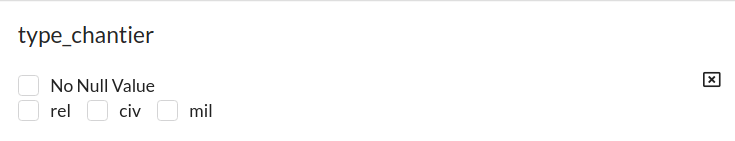
\includegraphics[width=0.8\linewidth]{OriginalPaperstatic/figures/ComBiNet/OriginalPaperFigures/categoricalWidget}
    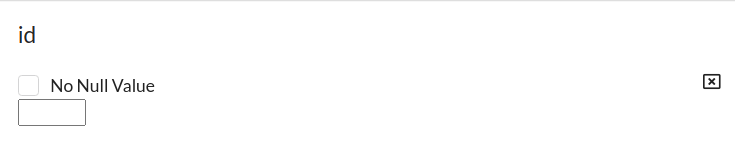
\includegraphics[width=0.6\linewidth]{static/figures/ComBiNet/OriginalPaperFigures/nominalWidget}
    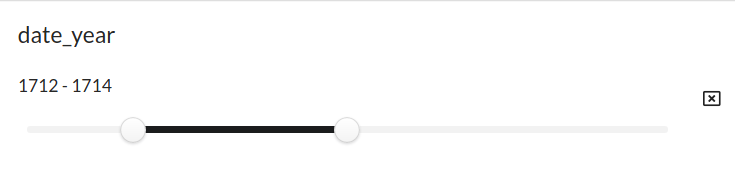
\includegraphics[width=0.6\linewidth]{static/figures/ComBiNet/OriginalPaperFigures/numericWidget}


    \caption{Widgets are associated with the three different attribute types: categorical (top), nominal (middle), numeric (bottom). The categorical widget shows the contextual menu with input buttons to create new widgets on other attributes or other nodes.}\label{fig:widgets}
\end{figure}

To answer our collaborator's question 2, we want to filter the documents which are located in Torino. For this, we first select the whole dataset by linking a person and document node with an \textit{any} link. Then, we select the id \textit{doc1} of the document of our visual node-link query, and the \textit{region} attribute. It will initialize a categorical widget including all the values found in the dataset for this attribute with associated checkboxes. We check the region of interest ``\textit{1-Turin Ville}'' to select all the documents from this region. The first widget of \autoref{fig:widgets} illustrates the created constraint along with the input buttons which allow the creation of new constraints.

% \begin{figure}
%     \centering
%     \includegraphics[width=0.8\linewidth]{OriginalPaperstatic/figures/ComBiNet/OriginalPaperFigures/constraintRegion.png}
%     \caption{Attribute constraint on the attribute \textit{region} of the document node \textit{d}. Only the documents from the region \textit{Turin-Ville} will be returned. \jdf{Tu pourrais mettre ce widget dans la figure au dessus pour éviter d'avoir deux figure ? C'est un bon exemple de contraintes catégorielles.}}\label{fig:constraintTurin}
% \end{figure}


\noindent\textbf{V8: Cypher Editor}
Users can build or modify a query using the Cypher query language, with the Cypher text editor. This allows users to start creating a query visually, and refining it by text for complex constraints which can not be represented by a visual form easily. The visual and textual representations are synchronized, meaning that changing one will update the other and update the results in the visualizations.


% \subsubsection{Results Panel}
\textbf{Query Results}
Each modification of the query, whether from the node-link dynamic query, the widgets, or the Cypher text boxes, update the two visualization panels (V1, V2), the entities tables (V3), the graph measures view (V5) and the attribute plots (V6).
The nodes and links that do not match (are not retrieved by the query) are grayed out in V1 and V2, and are removed from the persons and documents tables (V3). A third table shows every found occurrence of the created pattern. Users can switch between tables in the table view with tabs.
The graph measures are computed on the new graph formed by the union of all patterns found and updated on the graph measures view (V5). Since some measures can be long to compute, the values are computed iteratively and shown in a progressive manner \cite{fekete2019progressive} to not block the interface.
The distribution plots in the attributes view (V6) are updated, now showing the values of the entities of the new pattern, next to the global distributions.


% Each modification of the query, whether from the node-link dynamic query, the widgets, or the Cypher text boxes, update the two visualization panels. The nodes and links that do not match (are not retrieved by the query) are grayed out. It allows to rapidly visualize the subset of entities resulting from the applied query while maintaining the context.
% The results are shown in detail in the results section panel, constituted of the results tables and summary tabs, both shown in \autoref{fig:ResultsSection}. The table shows each occurrence of the query pattern found in the graph, with details on demands. Clicking on a row shows every attribute of the matched entities. Users can select a set of rows to highlight and visualize the occurrences directly in the two graph views.

% The summary tab presents graph measures computed from the subgraph resulting from the union of all occurrences of the queried pattern, such as the number of persons, documents, bipartite density, and the bipartite clustering coefficient. For the specified query, 42 documents are localized in Torino, 99 persons are mentioned in these contracts 153 times (given by the number of links).



\begin{figure}
    \centering
    %\begin{}

    % \begin{subfigure}[b]{0.30\linewidth}
    % 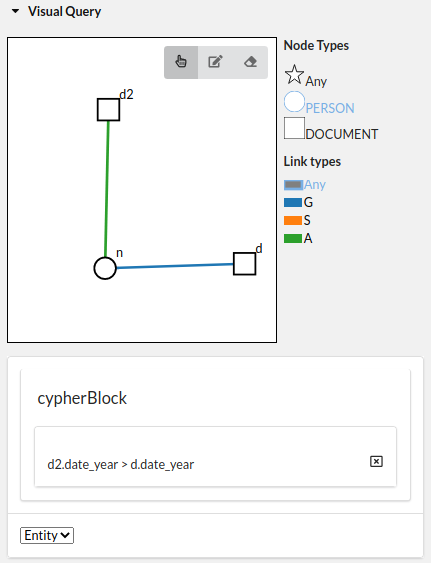
\includegraphics[width=\textwidth]{OriginalPaperstatic/figures/ComBiNet/OriginalPaperFigures/sankeyQuery.png}
    % \caption{}
    % \end{subfigure}
    % \begin{subfigure}[b]{0.30\linewidth}
    % 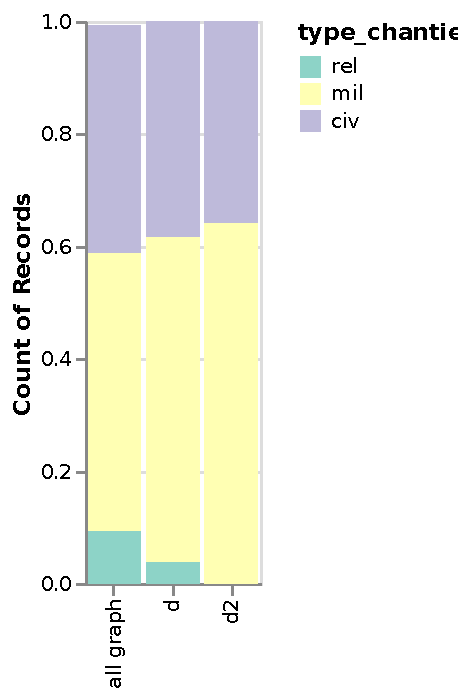
\includegraphics[width=\textwidth]{OriginalPaperstatic/figures/ComBiNet/OriginalPaperFigures/typeChantierSankeyQuery.pdf}
    % \caption{}
    % \end{subfigure}
    % \begin{subfigure}[b]{0.30\linewidth}
    % 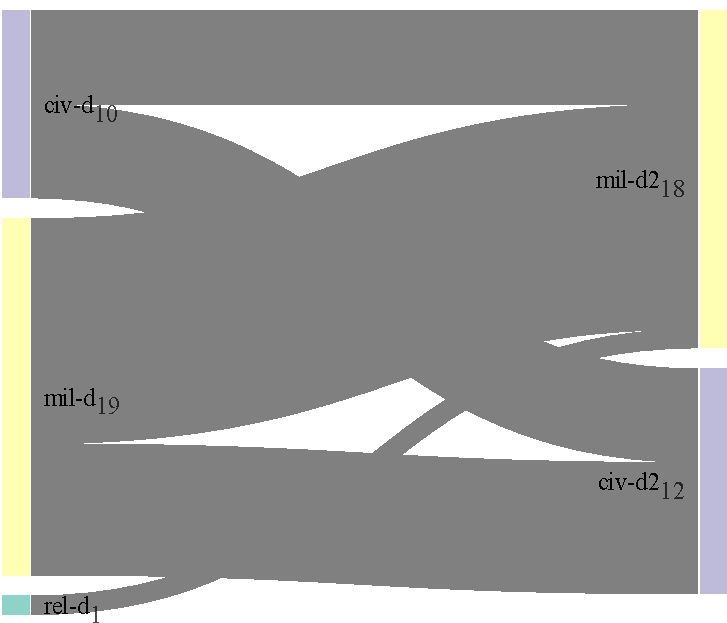
\includegraphics[width=\textwidth]{OriginalPaperstatic/figures/ComBiNet/OriginalPaperFigures/sankeyTypeChantier.pdf}
    % \caption{}
    % \end{subfigure}

    \begin{subfigure}[b]{0.30\linewidth}
        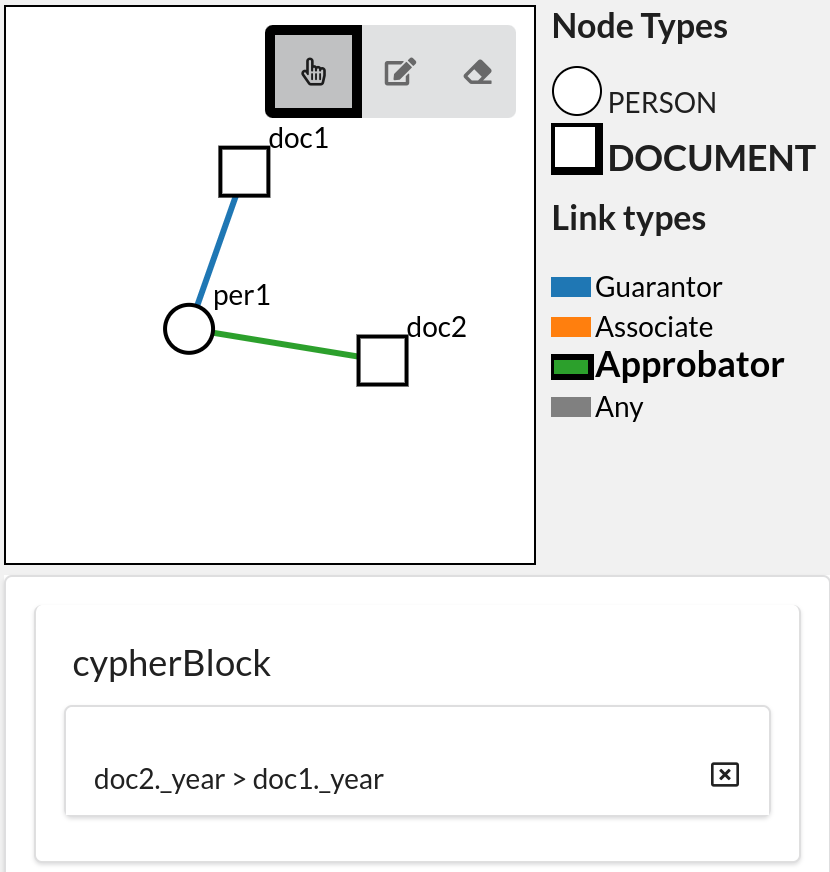
\includegraphics[width=\textwidth]{static/figures/ComBiNet/OriginalPaperFigures/CGF/sankeyPLot/apprGuar.png}
        \caption{}
    \end{subfigure}
    \begin{subfigure}[b]{0.30\linewidth}
        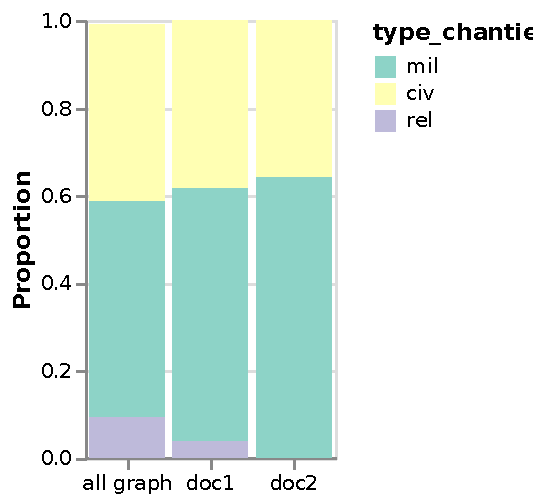
\includegraphics[width=\textwidth]{static/figures/ComBiNet/OriginalPaperFigures/CGF/sankeyPLot/barchart.pdf}
        \caption{}
    \end{subfigure}
    \begin{subfigure}[b]{0.33\linewidth}
        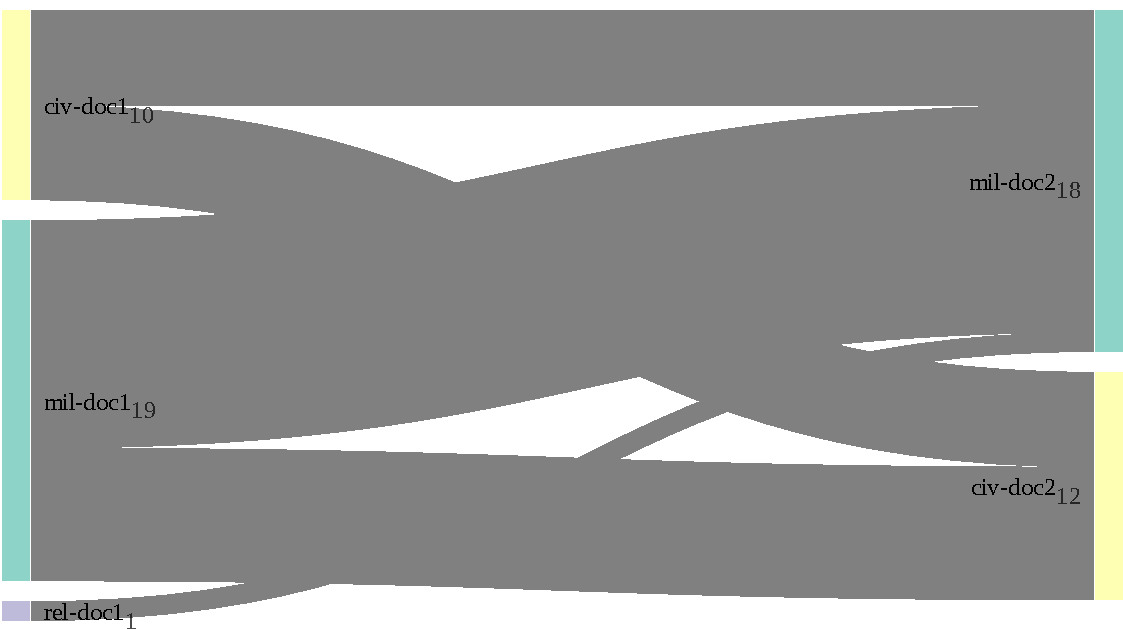
\includegraphics[width=\textwidth]{static/figures/ComBiNet/OriginalPaperFigures/CGF/sankeyPLot/sankey_bigger.pdf}
        \caption{}
    \end{subfigure}

    \caption{Two ways of showing the distribution of ``type chantier'' (type of works), a categorical attribute with three possible values ``\textsl{rel}igious'', ``\textsl{mil}itary'', and ``\textsl{civ}ilian''.
        (a) A query matching all the contracts made by the same person ($n$) as an ``approbator'' (green link to $d2$) after being a ``guarantor'' (blue link to $d$) using the time constraint (\texttt{d2.\_year > d.\_year}). (b) Stacked bar chart for the overall matches, the earlier of the two contracts ($d$), and the older contract ($d2$), and (c) Sankey diagram with the early values on the left and the older values on the right.
        The Sankey diagram reveals the change of values between the two documents: the guarantor who worked initially on religious work ended up working on a military work.} \label{fig:sankeys}
\end{figure}

% \textbf{Attributes Visualization.} To the right of the summary table, users can select or hover an attribute name to show its distribution in two contexts: the whole graph and the matched entities for the specified query. Categorical attributes appear as stacked bar charts while numeric attributes are shown as area charts. It allows characterizing in detail the group of nodes returned by the query according to the attributes the user is interested in. It shows if there are differences or correlations between several entities, and how they relate to the overall distributions.

\textbf{Attributes Visualization.} When users select an attribute in the attributes view (V6), it shows its distribution for the whole network and the query's entities.  However, these plots show the aggregated values and we lose the potential value transitions between the nodes of the query.
For example, \autoref{fig:sankeys} shows a query to list the persons who had a role of ``approbator'' (noted ``A'' in green) in a contract after being a ``guarantor'' (marked ``G'' in blue) in another contract (using a time constraint). We may want to see if the locations or type of the two contracts are the same or if they change, case by case. Unfortunately, we lose this information with the aggregated plots. By checking the ``Sankey'' option on top of the distribution visualization, the plots are transformed into Sankey diagrams, giving information on how the attribute values relate between the nodes (person or event) of the same query.
% The given query example along the distribution of the \textit{type chantier} in both a stacked bar chart and Sankey diagram is shown in .
A Sankey diagram for showing the attribute distributions is particularly useful for queries where the nodes have time relationships by definition, such as birth certificates, marriage, or death certificates where we know the order in which these events occurred. It is also useful for queries with user defined time order constraints as in \autoref{fig:sankeys}.


% The two tabs of the results panel after we applied our filters are shown in \autoref{fig:ResultsSection}.


% \begin{figure}
%     \centering
%     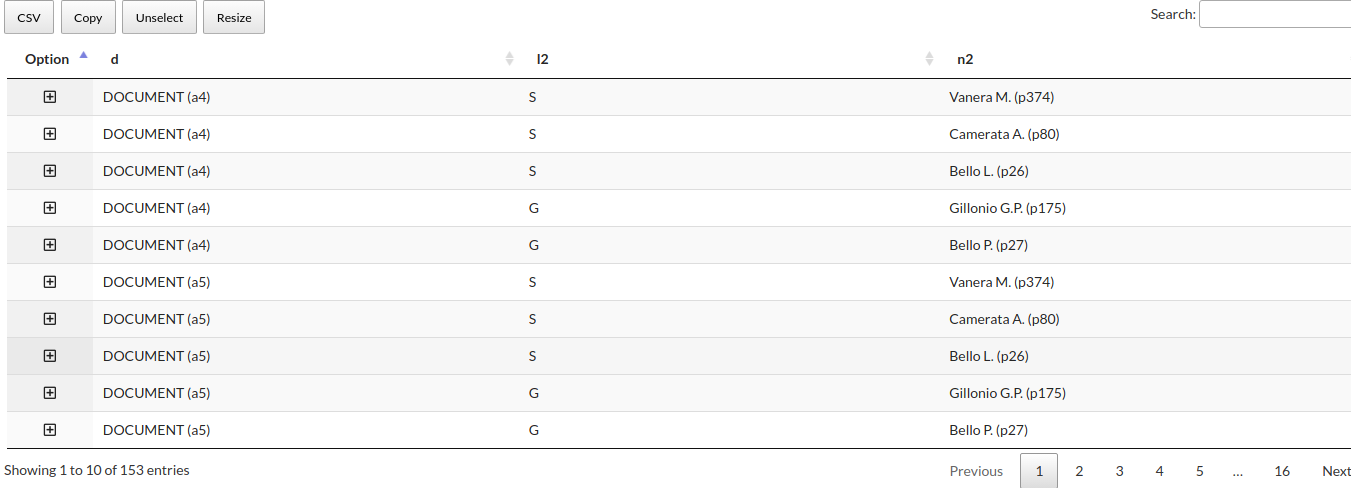
\includegraphics[width=0.99\linewidth]{OriginalPaperstatic/figures/ComBiNet/OriginalPaperFigures/TableExample}
%     \caption{The table tab of the result panel shows every pattern which matched with the constructed query. Clicking on the plus button shows details on the matched nodes, and users can select specific occurrences to highlight them in the graph view and center the view around them.}\label{fig:ResultsSection}
% \end{figure}

% \begin{figure}[b]
%     \centering
%     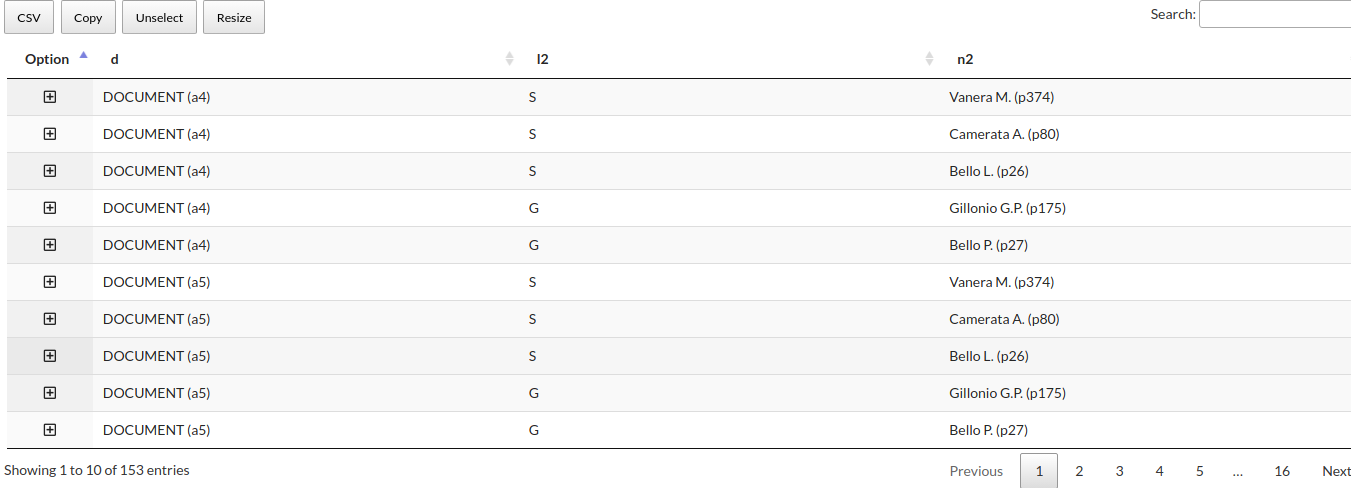
\includegraphics[width=0.99\linewidth]{OriginalPaperstatic/figures/ComBiNet/OriginalPaperFigures/TableExample}
%     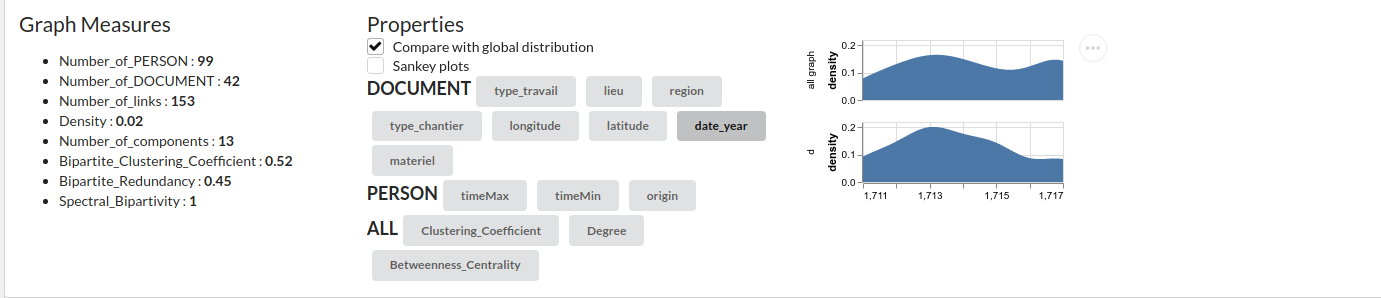
\includegraphics[width=0.99\linewidth]{OriginalPaperstatic/figures/ComBiNet/OriginalPaperFigures/SummaryExample}
%     \caption{The detailed results panel shows a table (top) and summary tab (bottom) of the request specified in the query panel. The table shows each match of the query, while the summary presents graph measures for the graph elements matching the query, along with the distributions of the attributes. Here, the user selected the \textit{date\_year} attribute; the distributions show that the distribution of the selection is similar to the distribution of the whole graph.}\label{fig:ResultsSection}
% \end{figure}

\noindent\textbf{V9: Provenance Tree}
Each change in the query panel is saved with the computed results, so that the history of the query construction can be shown in the form of a provenance tree (T2.4), managed using the Trrack library~\cite{cutler_trrack_2020}. Each node of the tree represents a change in the query, with a description label like ``New Link'' for the creation of a new link. It allows to rapidly visualize the succession of filters applied with their refinements. At any moment, users can click on a node of the tree to go back to a previous query state. It allows reverting to a satisfactory state if a change resulted in disappointing results. Hovering over a node of the tree shows a tooltip with its query visualization. If a change is done after reverting to a previous state, a new branch is created on the tree, allowing to go back to a previous interesting query and refine it in an exploratory way.  \autoref{fig:teaser} shows the provenance tree at the bottom of the query panel.


%  \autoref{fig:provenanceTree} shows the provenance tree of the two previous applied filters.

% \begin{figure}
%     \centering
%     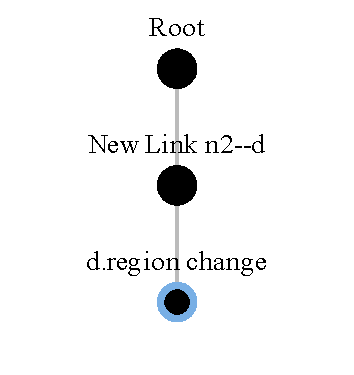
\includegraphics[height=3cm]{OriginalPaperstatic/figures/ComBiNet/OriginalPaperFigures/provenanceTree}
%     \caption{Provenance tree of the query formalized in  \autoref{sec:attributes} \todo{add a tree with several branches}}\label{fig:provenanceTree}
% \end{figure}

\subsection{Comparison}

In addition to comparing the results of a query to the whole graph, \name allows comparing the results of two queries.
% We now present the different interaction techniques implemented to allow the comparison between two query results.
Users can select query states in the provenance tree and mark them either as "A" or "B". They can click on the button ``Compare State A and B'' to compare the two query results. The interface changes to \textit{comparison mode}. Several buttons appear on top of the provenance tree: $A$, $B$, $A-B$, $B-A$, $A \cap B$, $A \cup B$ for showing various combinations of the two results of A and B, in the two visualizations panels.

% The user can select a history point in the provenance tree to compare it to the current query state, which we name ``query A''. The query associated with the history point in the tree  is named ``query B''. The interface changes to \textit{comparison mode}. Several buttons appear on top of the provenance tree: $A$, $B$, $A-B$, $B-A$, $A \cap B$, $A \cup B$ for showing various combinations of the two results of A and B.

To answer several of the questions raised by our collaborators, we need to compare two subsets of the network.
% Similarly to a lot of questions our collaborators gave us, we have to compare two subsets of the graph to answer our current use case :
For the question 2 from \autoref{tab:tasks}, we want to compare the works in \textit{Turin} with the ones in \textit{Turin Territoire}. Since we previously constructed the query returning all the contracts from \textit{Turin} with the mentioned people, we can
return to this point, change the constraint of the \textit{region} attribute from \textit{Turin} to \textit{Turin Territoire} using the checkbox to get the two queries we want to compare. They are shown in \autoref{fig:visualQueriesExamples}.

% To answer the question or our user, we will compare the query describe in the previous section with a similar query where this time the \textit{region} attribute of the node \textit{d} is equal \textit{Turin Territoire}.

% \begin{figure}
%     \centering
%     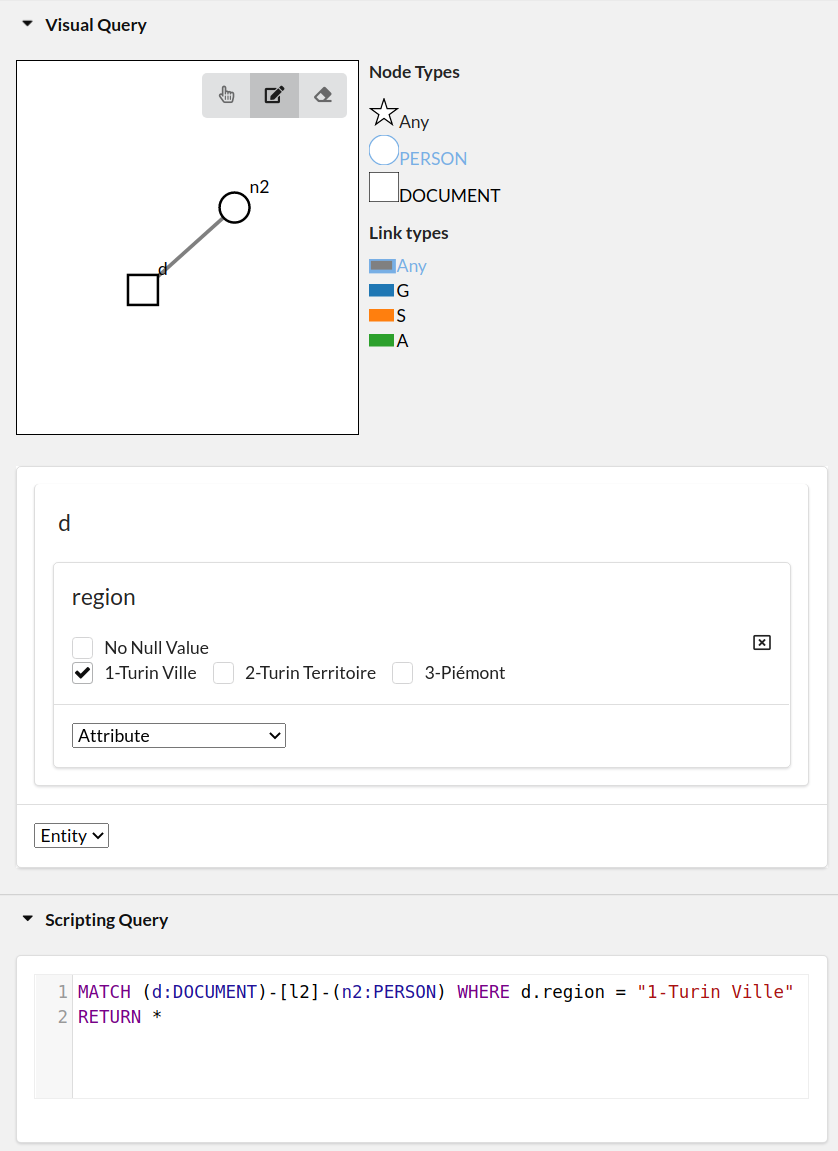
\includegraphics[width=0.49\linewidth]{OriginalPaperstatic/figures/ComBiNet/OriginalPaperFigures/visualQueryTurin}
%     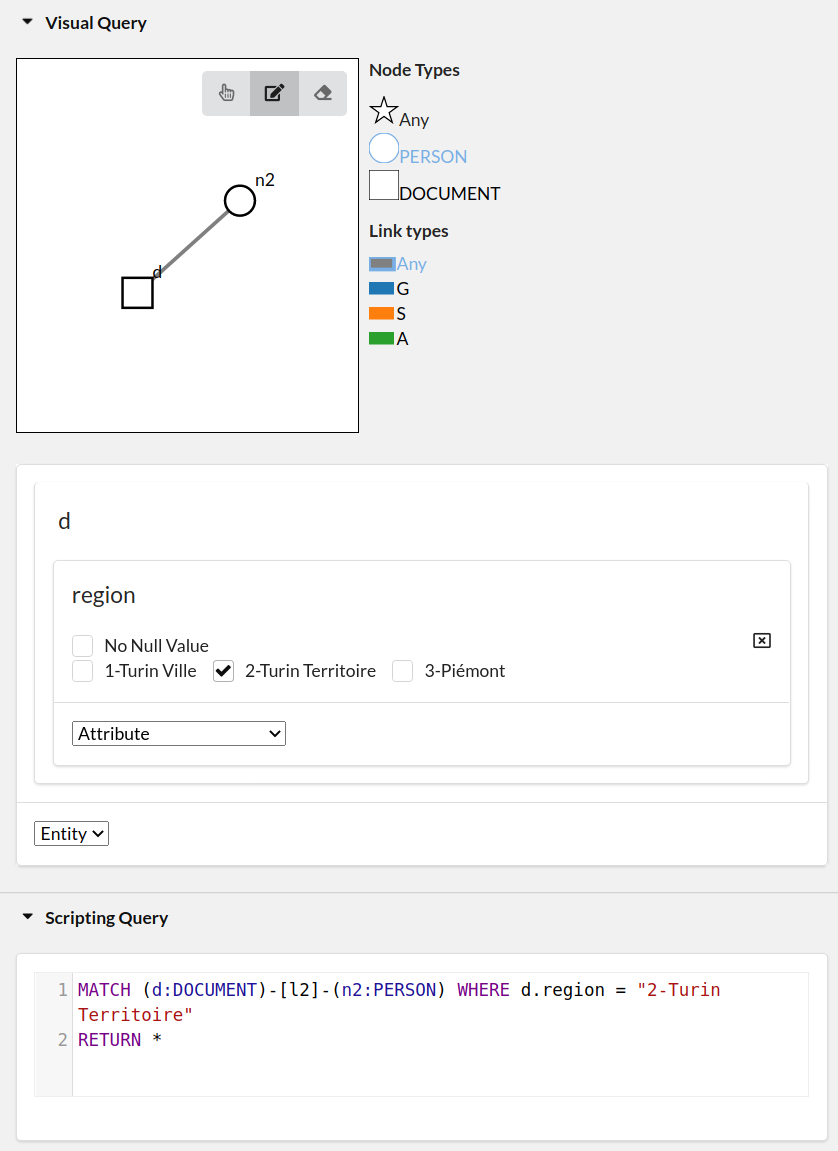
\includegraphics[width=0.49\linewidth]{OriginalPaperstatic/figures/ComBiNet/OriginalPaperFigures/visualQueryBanlieue}

%     \caption{The two visual queries created by the user to retrieve the documents---along with the signatories---of \textit{Turin} (left) and of \textit{Turin Territoire} (right).}\label{fig:queriesToCompare}
% \end{figure}

% \begin{figure}
%     \centering
%     % \includegraphics[width=0.2\linewidth]{OriginalPaperstatic/figures/ComBiNet/OriginalPaperFigures/query01.png}
%     % \includegraphics[width=0.2\linewidth]{OriginalPaperstatic/figures/ComBiNet/OriginalPaperFigures/query02.png}
%     % \includegraphics[width=0.2\linewidth]{OriginalPaperstatic/figures/ComBiNet/OriginalPaperFigures/query03.png}
%     % \includegraphics[width=0.2\linewidth]{OriginalPaperstatic/figures/ComBiNet/OriginalPaperFigures/query04.png}
%     \includegraphics[scale=0.1]{OriginalPaperstatic/figures/ComBiNet/OriginalPaperFigures/CGF/MutualGuarantors.png}
%     \includegraphics[scale=0.1]{OriginalPaperstatic/figures/ComBiNet/OriginalPaperFigures/CGF/Turin.png}
%     \hspace{-8pt}
%     \includegraphics[scale=0.1]{OriginalPaperstatic/figures/ComBiNet/OriginalPaperFigures/CGF/TurinoSuburbs.png}
%     \caption{Queries to answer our collaborator's four questions.
%     % Visual queries made to find back the four patterns our collaborator is interested in.
%     }\label{fig:queries}
%     \vspace{-8pt}
% \end{figure}

\begin{figure}
    \centering

    \begin{subfigure}{0.22\linewidth}
        \centering
        \includegraphics[width=\textwidth]{static/figures/ComBiNet/OriginalPaperFigures/CGF/MutualGuarantors.png}
        \caption{}
    \end{subfigure}
    \hspace{8pt}
    \begin{subfigure}{0.70\linewidth}
        \centering
        \includegraphics[width=0.46\textwidth]{static/figures/ComBiNet/OriginalPaperFigures/CGF/Turin.png}
        \includegraphics[width=0.46\textwidth]{static/figures/ComBiNet/OriginalPaperFigures/CGF/TurinoSuburbs.png}
        \caption{}
    \end{subfigure}

    \caption{The two visual queries created by the user to retrieve the documents---along with the signatories---of \textit{Turin} (left) and of \textit{Turin Territoire} (right).} \label{fig:visualQueriesExamples}
\end{figure}

\noindent\textbf{Topological Comparison}
In visualization mode, the two graph visualization panels do not change but users can rapidly change between the visual filter of (A) and (B) by hovering over their respective buttons on the comparison menu and thus rapidly comparing the structure of the two resulting subgraphs (T3.1). Similarly, different Boolean comparison operations are available through hovering their respective buttons (shown in \autoref{fig:teaser}-C), such as the intersection, union, and differences of the two filters. % It allows to rapidly change filters to find interesting persons or group of persons in a exploratory process.
Moreover, the summary tab on top of \autoref{fig:teaser}-D allows comparing the different graph measures of the two subgraphs by showing them side by side in a table layout (T3.3).
% as shown in \autoref{fig:comparisonTable}.
Comparing these measures, such as the number of matched documents or the bipartite density is interesting information in SNA.

\iffalse
\begin{figure}
    \centering
    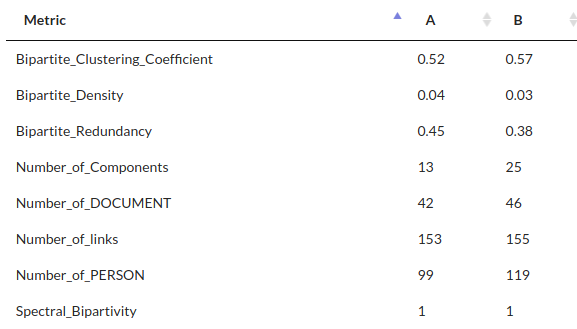
\includegraphics[width=0.8\linewidth]{static/figures/ComBiNet/OriginalPaperFigures/comparisonPlots/graphMeasuresComparison.png}
    \caption{Comparison table of the graph measures of the query filters (A) and (B)}\label{fig:comparisonTable}
\end{figure}
\fi

\noindent\textbf{Attribute-Based Comparison}
The comparison of one or several attribute distributions between (A) and (B) is often more useful to answer the historical questions of our users. In the attribute view of the results panel, hovering or clicking on an attribute name will show the distribution of this attribute in four contexts: the nodes of the whole graph, of the queries (A), (B), and the currently selected Boolean operator (e.g., intersection or union). This allows user to compare attribute distributions between several subsets of interest (T3.2). For example, we can compare the attributes between the contracts of Torino and the ones of its close territory. We can also compare the persons who worked in Torino, in Torino's close territory, and in both areas, by selecting the intersection operator.
% or the persons who collaborated in those regions, if we select the intersection operator.
\autoref{fig:attributeComparison} illustrates the comparison charts for different attributes.  We can see that the types of construction sites differ between the two regions: the city of Torino clearly have a lot of military sites compared to the territory of Turin which has almost none. This is the reverse for the number of religious sites, which are almost all localized in the territory of Torino. If we now look at the year distribution of the contracts, we can see a difference in the spike of the distributions. The majority of Torino's contracts have occurred around 1713 and around 1717 for Torino's territory.
We can also compare the profile of persons who collaborated both at Torino and Torino's territory by selecting the intersection of those two queries. One of the questions the historian had (question 2 of \autoref{tab:tasks}) was to know if those persons were a group with specific attributes and characteristics, or were inseparable from other persons working in the two areas. If we look at the betweenness centrality, on average, the values are higher for this group of people, meaning that the persons who work in the construction site at Torino and Torino's territory are clearly two distinct groups, and the persons collaborating in the two areas act as bridges between these groups.
This visual demonstration was convincing and revealing for our users.

\begin{figure}
    \centering

    % \includegraphics[width=0.2\linewidth]{OriginalPaperstatic/figures/ComBiNet/OriginalPaperFigures/comparisonPlots/type_chantier}
    % % \includegraphics[width=0.2\linewidth]{OriginalPaperstatic/figures/ComBiNet/OriginalPaperFigures/comparisonPlots/type_travail}
    % 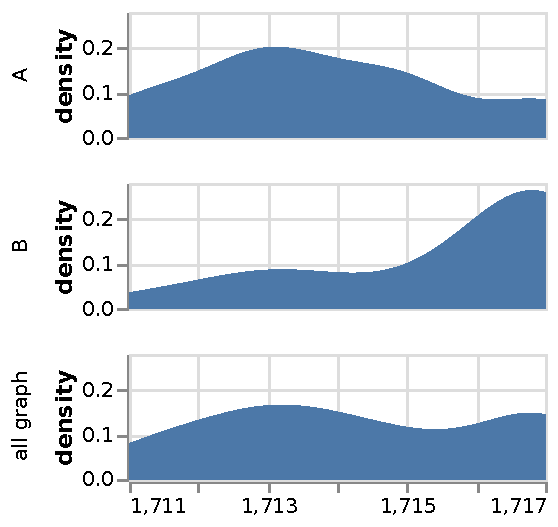
\includegraphics[width=0.2\linewidth]{OriginalPaperstatic/figures/ComBiNet/OriginalPaperFigures/comparisonPlots/date_year}
    % 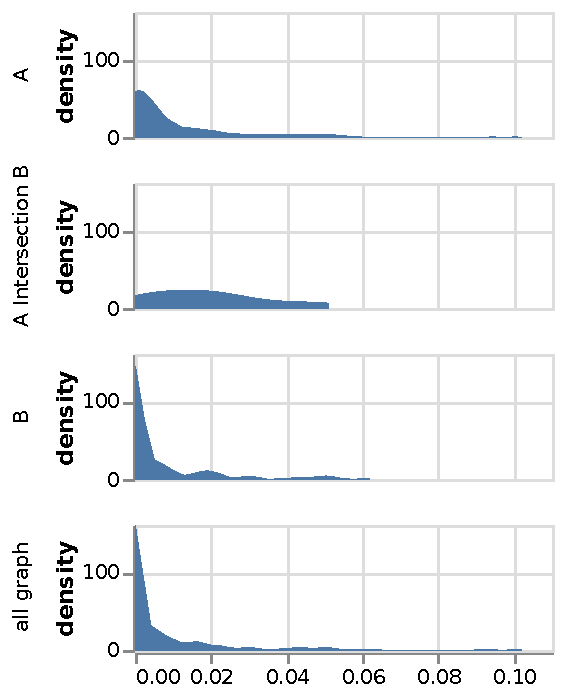
\includegraphics[width=0.2\linewidth]{OriginalPaperstatic/figures/ComBiNet/OriginalPaperFigures/comparisonPlots/Betweeness_Centrality}

    % \includegraphics[height=90px]{OriginalPaperstatic/figures/ComBiNet/OriginalPaperFigures/comparisonPlots/type_chantier}
    % % \includegraphics[width=0.2\linewidth]{OriginalPaperstatic/figures/ComBiNet/OriginalPaperFigures/comparisonPlots/type_travail}
    % 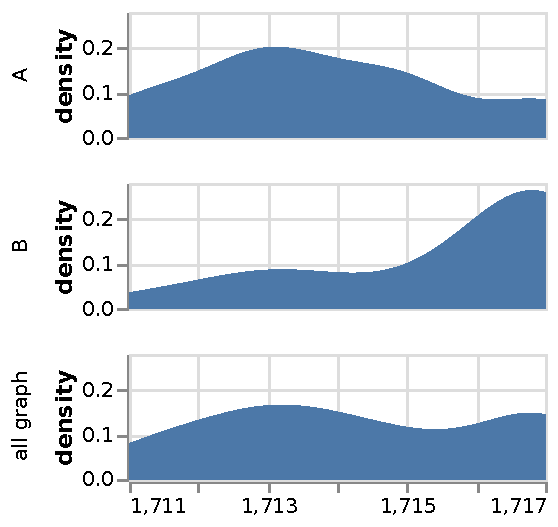
\includegraphics[height=90px]{OriginalPaperstatic/figures/ComBiNet/OriginalPaperFigures/comparisonPlots/date_year}
    % 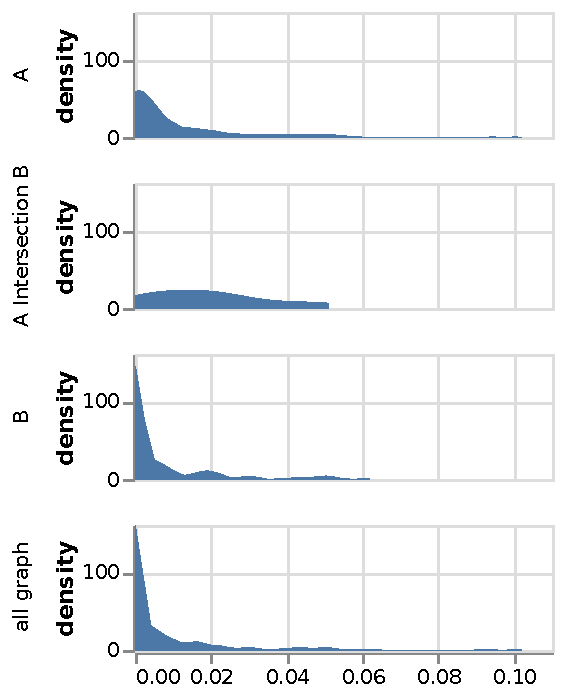
\includegraphics[height=90px]{OriginalPaperstatic/figures/ComBiNet/OriginalPaperFigures/comparisonPlots/Betweeness_Centrality}

    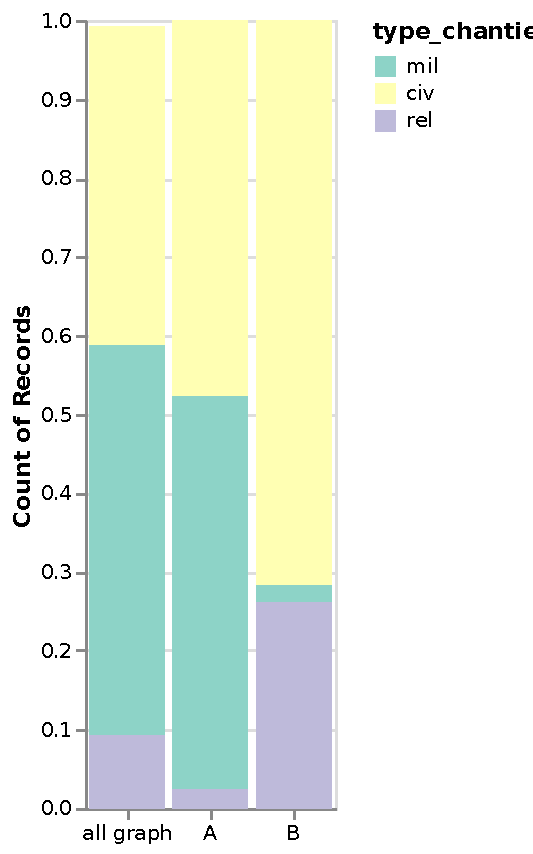
\includegraphics[height=60px]{static/figures/ComBiNet/OriginalPaperFigures/CGF/TurinPlots/type+chantier.pdf}
    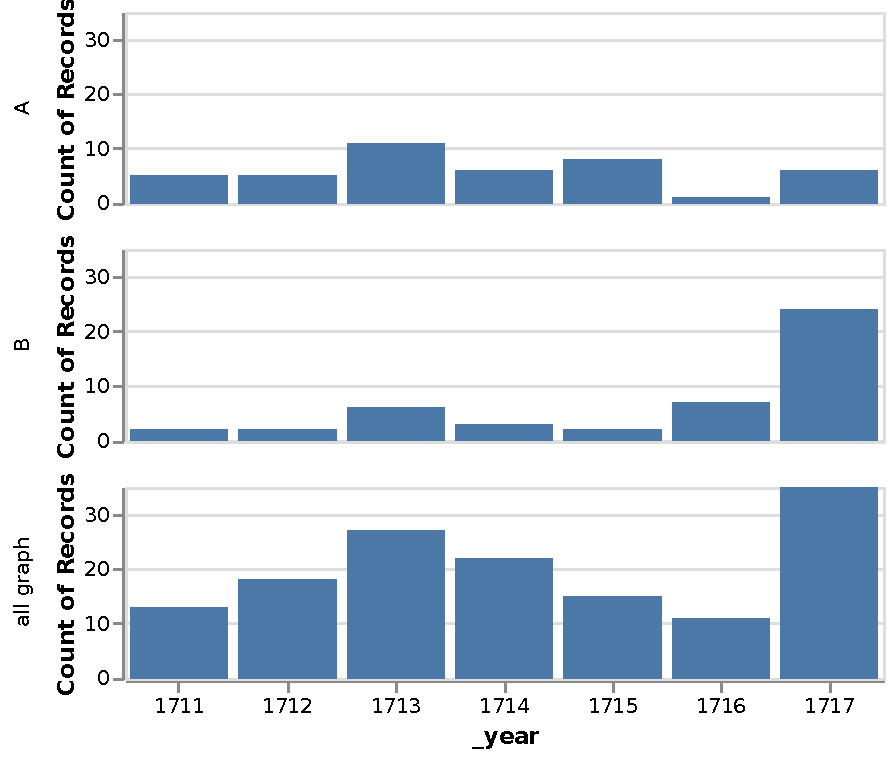
\includegraphics[height=60px]{static/figures/ComBiNet/OriginalPaperFigures/CGF/TurinPlots/time.pdf}
    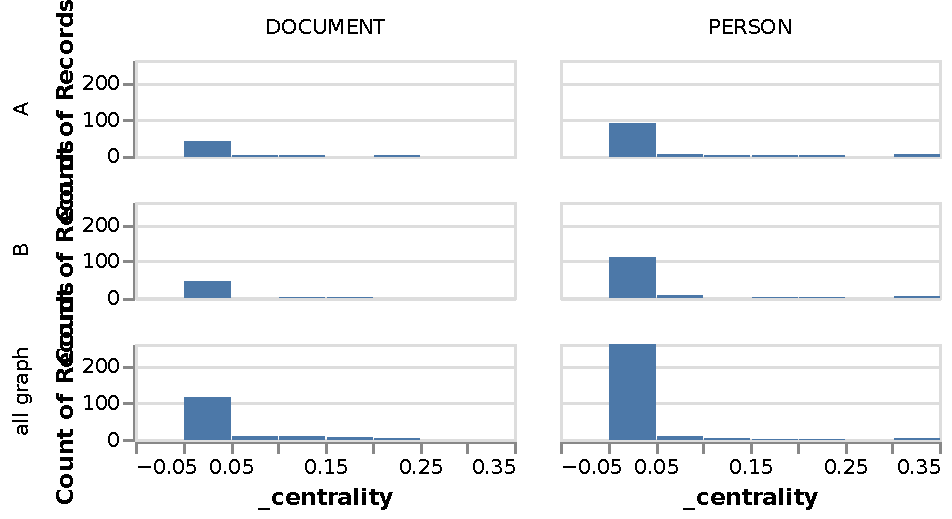
\includegraphics[height=60px]{static/figures/ComBiNet/OriginalPaperFigures/CGF/TurinPlots/centrality.pdf}


    \caption{Distribution of two document attributes and one global attribute for the documents and signatories of \textit{Turin} (A), \textit{Turin Territoire} (B) and the whole graph. (top).}\label{fig:attributeComparison}
\end{figure}


\subsection{Implementation}

\name is made of three components: a web visual interface, a python server, and a Neo4j graph database instance. The client interface is written in Javascript, using D3~\cite{d3}, Vega~\cite{satyanarayan2016vega}, and the Trrrack library~\cite{cutler_trrack_2020}. The python server is written in Flask, and interacts with the Neo4j instance for query processing.
% before sending the results to the front end.
We implemented our Cypher parser with the ANTLR parser generator~\cite{parr1995antlr}.
%, for the visualization of the queries synchronized with the Cypher script.

% The current implementation can be used with thousands of nodes and links. Above that limit, we will need to change the interaction to explicitly trigger the queries instead of running them implicitly at each interaction.




\section{Use Cases}\label{sec:usecases}

In this section, we describe step by step how our system has been able to specifically answer questions from our users.
Since usability issues have not been resolved yet, the tool was mostly operated by the developers working side by side with the collaborators to test the expressiveness of the queries and the value of the results visualizations. The tool was refined as needed along the way.

\subsection{Construction sites in Piedmont (\#1)}

One of the main questions of our collaborator was to compare two families which he knew played a big role in the structure of the network: the \textit{Menafoglio} and \textit{Zo} families (question 4 in \autoref{tab:tasks}). He was interested in knowing if there were differences in specialization in type of contracts and area of work for the core members of these families, and to what extent they were collaborating. Moreover, he was very interested in characterizing the group of people collaborating with both families.

To answer those questions, we first selected the core members of the \textit{Menafoglio family}, by checking the people known by the historian, and their close neighbors. Looking at the bipartite view (see Figure 1 of the supplementary material), we can see that the group is pretty dense with people collaborating a lot between them. Looking at the map, we can clearly see that the family has been mostly active in Piedmont outside of Torino and Torino's close territory. We also have a first view of the attribute distribution of the persons in the group and their contracts.

Then, we do the same query for the Zo family. We can keep the same topological filter, and replace the name filters with the core members of the Zo family known by the historian. We can see on the bipartite view (see Figure 2 of the supplementary material) that the group is smaller, and is on a different area in the graph. The map enriched with a selection of the \textit{region} attribute shows us that, contrary to the Menafoglio, the Zo have been more active in Turin and its close territory.

Let's now compare the two groups using the \textit{comparison mode} by selecting the two queries in the provenance tree. This opens the comparison menu to quickly navigate between the visual selection of (A), (B), and the set $A \cap B$ that interests our collaborator. The table showing the graph measures of the two subsets confirm what is shown visually: the Menafoglio group is more populated but less dense than the Zo family.

Our user is then interested in comparing the distribution of several attributes between the two groups. We can clearly see in \autoref{fig:useCasePascal} that the Menafoglio family is more specialized in military sites, while the Zo family is doing more civil constructions. This is confirmed by the ``material'' distribution that shows that the contracts of the Menafoglio are often using stones, whereas it is never the case for Zo contracts. Finally, the persons collaborating in the two groups have a betweenness centrality higher in average. This make sense as they act as bridges linking the two families.
% Moreover, we can see in detail the difference in the region of contracts of the two families.

% \begin{figure*}
%     \centering

%     \begin{overpic}[width=0.15\linewidth]{OriginalPaperstatic/figures/ComBiNet/OriginalPaperFigures/useCase01/queryMena.png}\end{overpic}
%     \begin{overpic}[width=0.15\linewidth]{OriginalPaperstatic/figures/ComBiNet/OriginalPaperFigures/useCase01/queryZo.png}
%     \end{overpic}
%     \begin{overpic}[width=0.6\linewidth]{OriginalPaperstatic/figures/ComBiNet/OriginalPaperFigures/useCase01/comparisonRegionNoZoom.png}
%     \end{overpic}

%     \caption{}\label{fig:useCasePascal}
% \end{figure*}


% \begin{figure*}
%     \centering

%     \begin{overpic}[width=\linewidth]{OriginalPaperstatic/figures/ComBiNet/OriginalPaperFigures/useCase01/queryAndComparePascal}

%      \put(30,14){\small Comparison}
%     %  \put(25, 22){\circled{\large A}}
%     \put(25, 4){\circled{\large I}}
%      \put(40, 4){\circled{\large II}}
%     \end{overpic}

%     \includegraphics[height=120px]{OriginalPaperstatic/figures/ComBiNet/OriginalPaperFigures/useCase01/attributes/materiel.pdf}
%     %  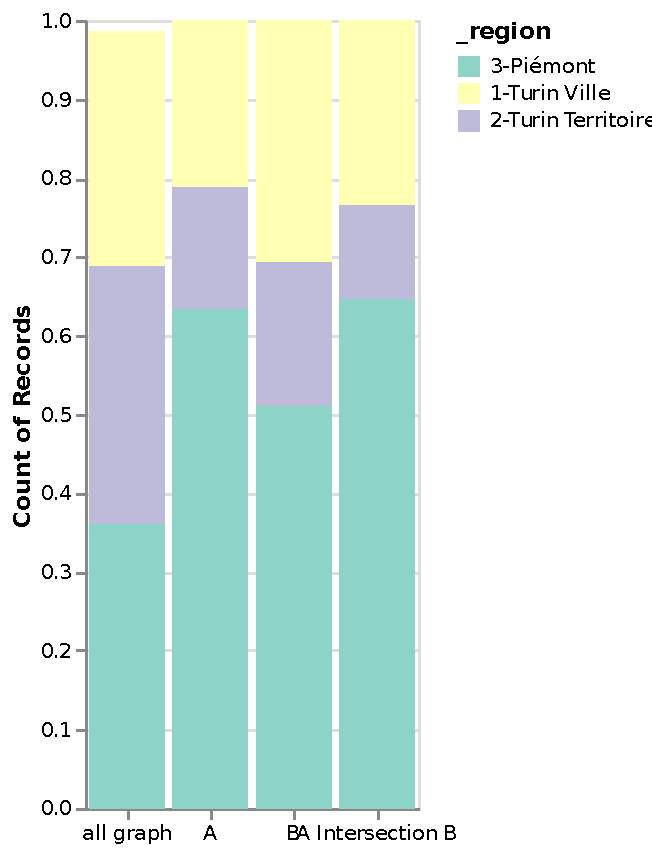
\includegraphics[width=0.2\linewidth]{OriginalPaperstatic/figures/ComBiNet/OriginalPaperFigures/useCase01/attributes/region.pdf}
%      \includegraphics[height=120px]{OriginalPaperstatic/figures/ComBiNet/OriginalPaperFigures/useCase01/attributes/type_chantier.pdf}
%      \includegraphics[height=120px]{OriginalPaperstatic/figures/ComBiNet/OriginalPaperFigures/useCase01/attributes/type_travail.pdf}
%      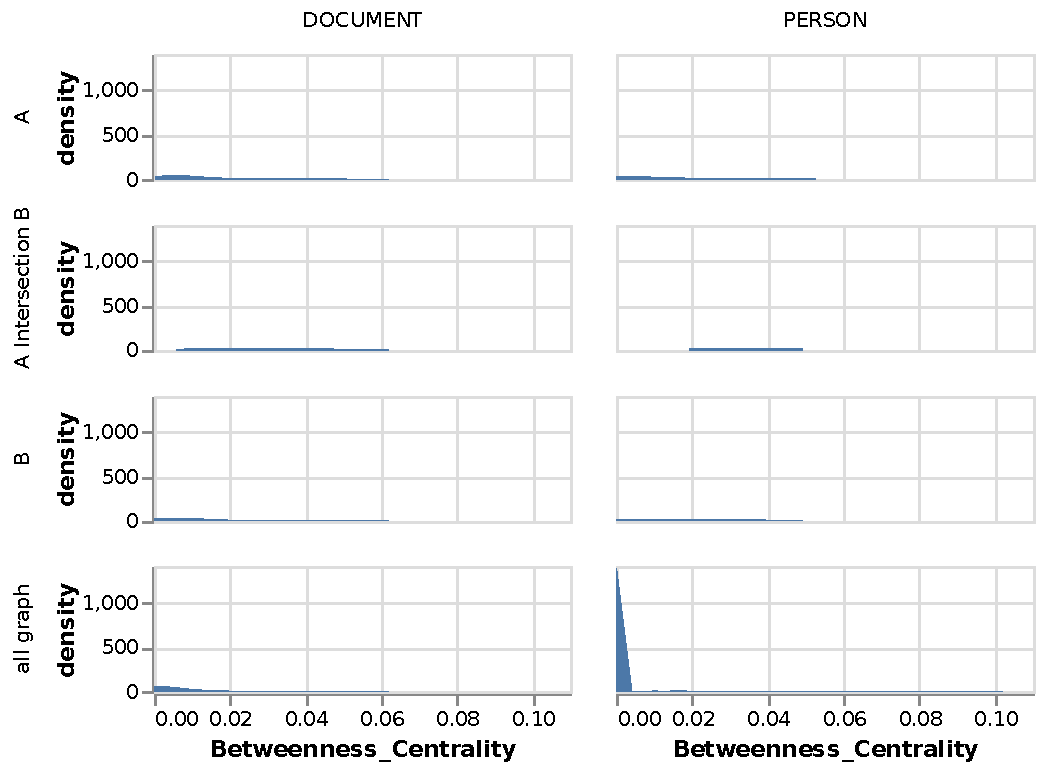
\includegraphics[height=120px]{OriginalPaperstatic/figures/ComBiNet/OriginalPaperFigures/useCase01/attributes/betweenness.pdf}

%     \caption{Comparison of the two group of interests for use case \pascal. (I) shows the two queries the user created to select the two groups of interest. (II) presents \name in comparison mode, with the intersection of (A) and (B) selected. The table shows the structural difference of the two groups, while the two graph views highlight the persons who collaborated between the two groups, who are of interest for our collaborator. The user selected the \textit{region} attribute, creating a plot showing that the Menafoglio and Zo families are working respectfully more in Piemont and Torino, while their collaboration has no strong associated region.}  \label{fig:useCasePascal}
% \end{figure*}

\begin{figure}
    \centering

    % \includegraphics[height=70px]{OriginalPaperstatic/figures/ComBiNet/OriginalPaperFigures/CGF/MenaZoPlots/materiel.pdf}
    %  \includegraphics[height=70px]{OriginalPaperstatic/figures/ComBiNet/OriginalPaperFigures/CGF/MenaZoPlots/type_chantier.pdf}
    %  \includegraphics[height=70px]{OriginalPaperstatic/figures/ComBiNet/OriginalPaperFigures/CGF/MenaZoPlots/type_travail.pdf}
    %   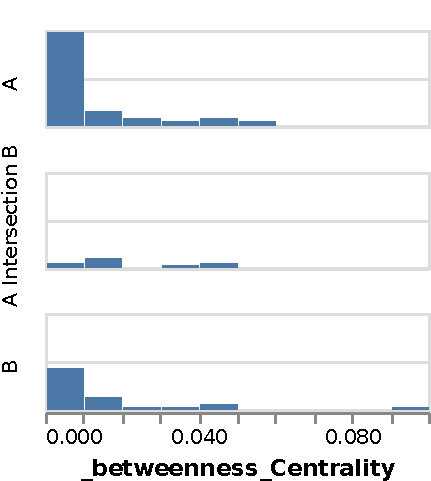
\includegraphics[height=80px]{OriginalPaperstatic/figures/ComBiNet/OriginalPaperFigures/CGF/MenaZoPlots/BC_crop.pdf}

    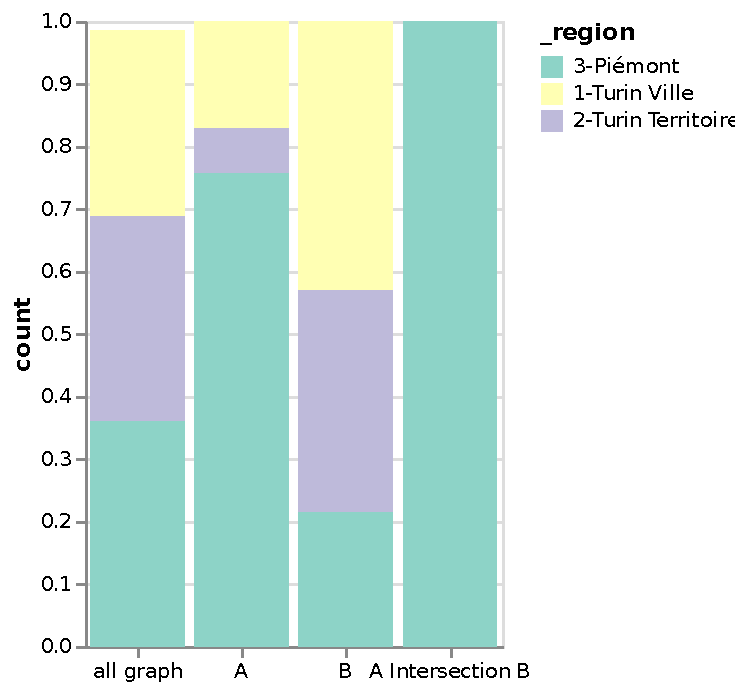
\includegraphics[height=50px]{static/figures/ComBiNet/OriginalPaperFigures/CGF/MenaZoPlots/v2/region.pdf}
    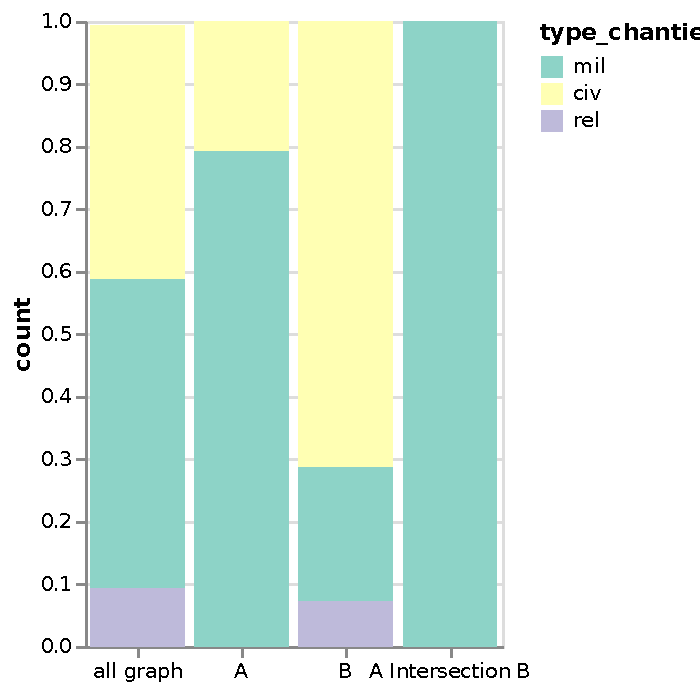
\includegraphics[height=50px]{static/figures/ComBiNet/OriginalPaperFigures/CGF/MenaZoPlots/v2/type-chantier.pdf}
    \includegraphics[height=50px]{static/figures/ComBiNet/OriginalPaperFigures/CGF/MenaZoPlots/v2/materiel.pdf}
    \includegraphics[height=50px]{static/figures/ComBiNet/OriginalPaperFigures/CGF/MenaZoPlots/v2/BC_crop.pdf}

    \caption{Attributes distributions plots between the whole graph, the \textit{Menafoglio} family (A), the \textit{Zo} family (B), and $A\cap B$, for the \textit{region,type\_chantier,  materiel type}, and \textit{betweenness centrality}  \label{fig:useCasePascal}}
\end{figure}


\subsection{French Genealogy (\#2)}

We describe how \name allowed to answer one of the main questions of our collaborator of the use case \nicole. She wanted to detect the largest migrations which occurred in several generations, and in which areas and at what time they happened (question 7 in \autoref{tab:tasks}).
The map view shows at a glance (see Figure 3 in the supplementary material) that the majority of events has taken place in three specific regions: one in the west of France, in the top-middle, and in the south-middle.

To find patterns of migrations inside families, we can first make a query representing a simple family by linking a person node to a birth event, itself connected to the parents using a link which is either of type \textit{father} or \textit{mother}. We then repeat the process on the new parent node to add another generation. Finally, we connect the latest generation child with a death event, to have another date and location to compare to (see \autoref{fig:UseCaseNicoleQ}). This query returns every person in the graph with their parents and grandparents, along with their respective birth data and death data for the latest person. We also create a constraint on the \textit{department} attribute on all document nodes to specify that we only want to retrieve the events that have an associated location and not a null value, as it is not often the case. This request returns a subgraph of 64 persons and 88 documents. The user can now select the \textit{department} attribute to create a Sankey diagram that shows the change of departments across the different generations of the returned families. \autoref{fig:UseCaseNicoleS} shows that the majority of families are from \textit{Haute-Vienne} (which can easily be confirmed by checking the map), and do not move much across generations. Our collaborator however detected interesting patterns of people moving from the department \textit{Creuse} to \textit{Haute-Vienne} across two generations. It interested her, so she refined the query by adding an attribute filter on this specific department using a widget. The table view then showed her who these migrant people were and when it occurred. The bipartite visualization panel allows exploring more in-depth this specific group of people. %, with their close neighbors.


% We now can use the Sankey visualization of the \textit{department} attribute to see if there is interesting patterns of migration.
\begin{figure}
    \centering
    % \begin{subfigure}{0.49\linewidth}
    % \includegraphics[width=\textwidth]{OriginalPaperstatic/figures/ComBiNet/OriginalPaperFigures/useCase02/queryParents3gen.png}
    % \caption{Visual query to find all 3-generation families (documents without department have been filtered out)}
    % \label{fig:UseCaseNicoleQ}
    % \end{subfigure}
    % % \includegraphics[width=0.4\linewidth]{OriginalPaperstatic/figures/ComBiNet/OriginalPaperFigures/useCase02/armorConstraint.png}
    % \begin{subfigure}{0.49\linewidth}
    % \includegraphics[width=\textwidth]{OriginalPaperstatic/figures/ComBiNet/OriginalPaperFigures/useCase02/sankey3genDep.pdf}
    % \caption{Sankey diagram showing the birthplace of people across generations and the death place}
    % \label{fig:UseCaseNicoleS}
    % \end{subfigure}

    \begin{subfigure}{0.49\linewidth}
        \includegraphics[width=\textwidth]{static/figures/ComBiNet/OriginalPaperFigures/CGF/frenchGenealogy/migrationQuery.png}
        \caption{Visual query to find all 3-generation families (documents without department value have been filtered out)}
        \label{fig:UseCaseNicoleQ}
    \end{subfigure}
    % \includegraphics[width=0.4\linewidth]{OriginalPaperstatic/figures/ComBiNet/OriginalPaperFigures/useCase02/armorConstraint.png}
    \begin{subfigure}{0.49\linewidth}
        \includegraphics[width=\textwidth]{static/figures/ComBiNet/OriginalPaperFigures/CGF/frenchGenealogy/migration3.pdf}
        \caption{Sankey diagram showing the birthplace of people across generations and the death place}
        \label{fig:UseCaseNicoleS}
    \end{subfigure}

    \caption{Migrations across departments over three generations}  \label{fig:useCaseNicole}
\end{figure}

Afterward, we answered the question 8 (see \autoref{tab:tasks}) of our user closely related to the first one. She wanted to compare the migrations in general between the 18th and 19th centuries. She thinks people really started moving in the 19th century and wanted to confirm it. To answer this, we first created a query to retrieve all the people with birth and death certificates from a specified department. We then applied a time filter on the death certificate node first for the 18th century and then the 19th century. We can then compare the two query results using the comparison mode, and look side by side at the Sankey graphs related to \textit{departments} as shown in \autoref{fig:useCaseNicole2}. We can clearly see that people do not move at all in the 18th century, while in the 19th century even if the majority of people stay in the same place from their birth to their death, we can still see more than half move. It thus confirms the hypothesis of our collaborator.

\begin{figure}
    \centering
    % \begin{subfigure}{0.49\linewidth}
    % \includegraphics[width=\textwidth]{OriginalPaperstatic/figures/ComBiNet/OriginalPaperFigures/useCase02/sankeyDep18c.pdf}
    % \caption{18th century}
    % \end{subfigure}
    % \begin{subfigure}{0.49\linewidth}
    % \includegraphics[width=\textwidth]{OriginalPaperstatic/figures/ComBiNet/OriginalPaperFigures/useCase02/sankeyDep19c.pdf}
    % \caption{19th century}
    % \end{subfigure}

    \begin{subfigure}{0.49\linewidth}
        \includegraphics[width=\textwidth]{static/figures/ComBiNet/OriginalPaperFigures/CGF/frenchGenealogy/migration_18.pdf}
        \caption{18th century}
    \end{subfigure}
    \begin{subfigure}{0.49\linewidth}
        \includegraphics[width=\textwidth]{static/figures/ComBiNet/OriginalPaperFigures/CGF/frenchGenealogy/migration_19.pdf}
        \caption{19th century}
    \end{subfigure}

    \caption{Sankey diagrams showing the migration of people in the 18th and 19th centuries, extracted from their birth and death place.}\label{fig:useCaseNicole2}
\end{figure}



% \subsection{Feedback}

% After a few iterations, we showed the final system to two of our collaborators during
% a three hours session. We answered their questions step by step while describing the process and the interface.
% They also took part in the analysis by asking new questions on their data, leading to new explorations and discussions.

% Both of them liked the Sankey view of the attributes, allowing them to see the evolution of distributions and answering several of their questions. Our collaborator of the use case \nicole\ was making sense of it by linking the migration patterns she was seeing in the Sankey view with specific persons of the dataset she knew in depth. She was also curious about other migration patterns she was not aware of, and wanted to know who these persons were, the system allowing her to select them and follow a deeper exploration.

% Both liked the export capabilities of the system to collect results in CSV or JSON format, as well as the charts in SVG, for inclusion in their publications or for processing with other tools.


\section{Usability Study}\label{sec:usability}

\subsubsection{Procedure}

After showing our tool can be used to answer socio-historical questions, we performed a formative usability study with two historians and one expert in visualization. We had 3 meetings with each, and gave them control of the tool to see if they can use it to explore their data, perform queries and comparisons. At each meeting, we asked them to speak aloud, commenting their aims and actions. At the end of each session we asked them their general feedback and what other features they would like to have. We improved the system and made the changes asked by the users before setting up new appointments. This usability study led to the revamp of some core features, like the activation of the comparison mode which is now started by first marking the state nodes in the provenance tree. It also led to the implementation of new features, such as the person and document tables (which are updated after each query), the persistent selection of nodes across the two views and the tables, and the undo feature for visual queries.
% The list of all feedback and modifications are shown in the supplementary material.
At the final meetings, the three users were able to perform exploration, queries and comparisons to answer socio-historical questions.

\subsubsection{Feedback}

Both historians liked the Sankey view of the attributes, allowing them to see the evolution of distributions and answering several of their questions. Our collaborator of the use case \nicole\ was making sense of it by linking the migration patterns she was seeing in the Sankey view with specific persons of the dataset she knew in depth. She was also curious about other migration patterns she was not aware of, and wanted to know who these persons were, the system allowing her to select them and follow a deeper exploration.

Both liked the export capabilities of the system to collect results in CSV or JSON format, as well as the charts in SVG, for inclusion in their publications or for processing with other tools.





\iffalse
\section{Discussion}

Useful to social scientists provide a good trade-off between expressive power and simplicity compared to alternatives, either not expressive enough or too complex.

Compared to other systems:
\textbf{Jigsaw}: close on many aspects, also relies on a stable data model, but more expressive using attributes and roles. Yet, we do not handle general named entities that seem less important than for intelligence analysis; they can sometimes be emulated with attributes.

We applied it to other projects, such as research administration: publication and contracts visualization, and exploration.


\textbf{VERTIGo}: similar for queries, but VERTIGo is able to adapt to any data model, does not prescribe a data model, and handle attributes.

We want to distribute \name as an open-source tool and facilitate its use.

Still needs the help of a programmer to import data. Other systems, such as Gephi, provide plugins for that.

\jdf{Maybe} We need to improve the usability, most of the use cases have been done with the help of the authors.


Possible discussion points :
- Hard to evaluate
- No dynamic visualization
- A bit hard to do query on the orders of events
- Dirty data

\fi


\section{Discussion}

We discuss here several points of potential limitations.

\textbf{Scalability.} We assess the scalability in network size (number of nodes and links) with respect of the cluttering and readability of the network visualizations. Our biggest dataset from \zacarias\xspace is constituted of 7212 nodes (4886 persons and 2326 events) and 7790 links, after splitting the documents into birth and marriage event nodes. The system allows exploration of network of this size with a decent frame rate. Large networks are usually hard to read due to edge crossings \cite{shneiderman2006network}. \name allows to navigate large graphs with the node-link visualization using zoom \& pan and filtering with the query system. It let users focus on subsets of the data, one at the time.

\textbf{Generalizibility.} The system have been designed specifically for \model which model well a diversity of historical sources we encountered via our collaborations : marriage acts, birth/death certificates, construction/work contracts, census, migrations forms. However, there exist some special dataset cases where documents can have relationships with other documents, such as letters for example. The model and interface would have to be slightly changed to take into account document-to-document links for these datasets.
Moreover, \model can also be used to model other types of similar data, such as scientific publications or thesis data.
Bipartite networks are also used in various other disciplines, such as biology \cite{klamt2009hypergraphs} or chemistry \cite{konstantinova2001application}. \name could in theory be extended to these other application domains, by modifying the map view to show other geolocation data related to the entities of the network.

\textbf{Dynamic representation.} The current system allows to explore the dynamic aspect of the data by using a color scale which encode the time. Other layouts taking into account the time could be implemented in the future. The visual query system could also be extended by introducing more complex time constraints, such as in \cite{monroe2012exploring}.

% \textbf{Visual and textual queries} As visual queries systems can become overbloated and difficult to use as the power of expression increases, we decided to keep our query system easy to use, with the possibility of refining queries textually.

% \textbf{Methodology.}


\section{Conclusion and Future Work}

We presented \name, a system for exploring temporal social networks aimed at social scientists. It relies on modeling data as bipartite, multivariate, dynamic social networks where persons are linked to documents or events using a typed link that expresses a role.
We have successfully applied our data model to a wide variety of historical, sociological, genealogical datasets, and publication data.
Our tool \name relies on this data model to allow historians to explore their data and then answer their sociological questions using 1) dynamic queries on the network structure to highlight groups of interests, and 2) visual comparisons to contrast selected groups according to their structure, time, or any other attribute.
% \name supports dynamic queries that are translated in textual queries in the Cypher language, providing a mixed modality to query data.
The results can be visualized as a node-link diagram, a geographical map, graph measures, and distributions of values for the attributes.

We have shown that complex explorations and analyses were easy to perform, and validated our approach by describing two use cases among many more projects we are collaborating with.
%\name provides novel techniques to compare social networks through a combination of queries, navigation in the provenance tree, and Boolean combinations of query results.

By specifying a unifying data model and novel high-level visual and interactive tools for the comparison of topology, attributes, and time, we believe \name leads the way towards a new generation of highly interactive exploration tools applicable to analyze a wide variety of real social networks.

For future work, we need to improve the usability of \name, now that we know that the system is effective at exploring and analyzing real social networks. Our collaborators are eager to use it on their own and asked us to teach it to their students.

\name will be extended to support more SNA measures and computations such as clustering; it would create a new attribute containing a cluster identifier. However, we are more interested in providing more layout options for the graph to better highlight the time, such as the PAOvis technique~\cite{valdivia:hal-02264960}.
